\chapter{Experimental setup} 

\paragraph{} The Mainz Microtron Accelerator (MAMI), where the experiment is set up and the transverse asymmetry is measured, is briefly described in this chapter.  The description of the beam monitors used to measure the beam parameters is given a special consideration. Following an overview of the experimental hall, the detectors and the electronic devices used to acquire and process the data. 

\section{Overview of the Experiment} \label{FirstDescription}

To measure the Beam Normal Single Spin Asymmetry, a polarized beam of $ \SI{570}{\mega \electronvolt}$ is directed towards a  $^{12}C$ target that is $\SI{10}{\milli \meter}$ thick. The detectors are made up of two fused-silica bars coupled to 3 (detector B) and 8 (detector A) PMTs, which are used to gather the Cherenkov light released when an electron passes through the fused-silica. The detector are placed inside the two spectrometers of the A1 hall. Due to the high beam current ($ \SI{20}{\micro \ampere}$), which is above their operating
limits, the standard detectors of the spectrometers are not employed in this experiment. The experiment aims to measure the cross-section asymmetry between the two electron spin orientations. The PMT signals are collected and digitalized by the \textbf{NINO} board, after a threshold selection, and sent to the A1 control room computer, where the DAQ program collect the data together with all the data coming from the beam monitors. The produced  binary files are later analyzed by the analysis program, which is a significant part of the work done in the framework of the thesis. 
The data collected are divided in \textit{events} made by 4 \textit{sub-events} in sequence. Each event corresponds to a temporal window of $\simeq \SI{80}{\milli \second}$, where each sub-event is $\SI{20}{\milli \second}$ long. This structure into sub-events reflects the polarization sequence of the beam.
Unlike the majority of experiments in high energy physics, an event is not a single interaction, but is made by all the electrons interacting with the detectors during the specified time interval. The PMT counts and the beam monitor values are saved for each sub-event, along with their time length (measured in clock cycles by the NINO electronic board) and other values which are required to process beam monitor data. The general structure of the event is the shown in figure \ref{fig:EventStructure} 

\begin{figure}[hbtp] 
\centering
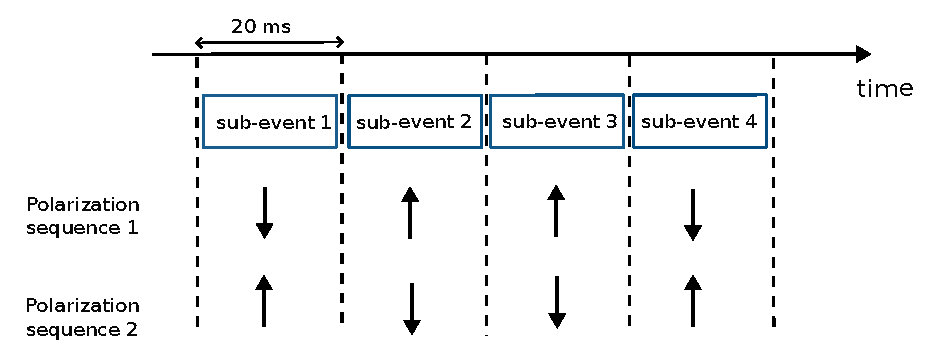
\includegraphics[width = 0.75\textwidth]{ExperimentalSetup/EventStructure.pdf}
\caption{General structure of the event. The gate-length of each event is synchronized with the power grid frequency, to reduce possible effects of $\SI{50}{\hertz}$ noise.}
\label{fig:EventStructure}
\end{figure}

The particular choice of $\SI{20}{\milli \second}$ for each sub-event is made to reduce undesirable effects relate to the power grid frequency ($\SI{50}{\hertz}$). The gate-length of each sub-events is synchronized with the period of the power grid frequency: this ensures that an entire oscillation of the current takes place within the same sub-event. This cancels out the $\SI{50}{\hertz}$ noise and avoid to produce effects between nearby sub-events.

An event corresponds to a single value measured of $A_{n}$, defined as the asymmetry between the $\uparrow$ and $\downarrow$ sub-events. To avoid the creation of false asymmetries by correlated noise or other external sources the polarization states are concatenated following the two patterns $\uparrow, \downarrow, \downarrow, \uparrow$ and $\uparrow, \downarrow, \downarrow, \uparrow$. Which sequence an event belongs to is decided using a De Bruijn sequence. A De Bruijn sequence of order n is defined as a cyclic sequence where every sub-sequence of length $n$ appears only once. We have two different polarization pattern, the ones shown in the figure, that can be represented as $1$ and $0$. For this experiment, the De Bruijn sequence is of order $n = 6$ bits, corresponding to all the possible sequences of $1$ and $0$ with a length equal to $6$, which are $64$ different sub-sequence.
It is possible to demonstrate that the number of exactly $N_{bruijn}$ sequences is: 
\begin{align*}
N_{bruijn} = \frac{(k!)^{k^{n-1}}}{k^{n}}
\end{align*}
If we substitute in the formula above $k=2$ and $n = 6$, we have a total of $\simeq 67 \cdot 10^{6}$ different sequences. The seed of the De Bruijn sequence is generated with a pseudo random number generator, and the sequence is used to select between $\uparrow,\downarrow,\downarrow, \uparrow$  and $\downarrow,\uparrow,\uparrow,\downarrow$. At this point it could be objected why so much care is taken in choosing randomly the two sequences. At a first glance is certainly easier to select one of the two polarization pattern and reproduce it for every sub-event. However, this would not protect from systematic effects that arise from electronic or beam noise with frequencies similar to the frequency of the polarization pattern. For instance electronic noise with  $ f \simeq \SI{10}{\hertz}$ could in principle increase the rates for one polarizations state and decrease the other one. The adopted solution to reduce effects of this type is to randomize the pattern selection. Besides this, there is another reason why a De Bruijn sequence is useful. During each polarization flip, we observe a short, transient reduction of the beam current. This reduction in the beam intensity has more influence on patterns where there are more inversion of the polarization respect to the other. With a De Bruijn sequence we ensure that we have a identical number of pairs of patterns, meaning that:

\begin{itemize}
\item $25\%$ : $\uparrow,\downarrow,\downarrow, \uparrow$ ; $\uparrow,\downarrow,\downarrow, \uparrow$
\item $25\%$ : $\downarrow,\uparrow, \uparrow,\downarrow$ ; $\downarrow,\uparrow, \uparrow,\downarrow$
\item $25\%$ : $\downarrow,\uparrow, \uparrow,\downarrow$ ; $\uparrow,\downarrow,\downarrow, \uparrow$
\item $25\%$ : $\uparrow,\downarrow,\downarrow, \uparrow$ ; $\downarrow,\uparrow, \uparrow,\downarrow$
\end{itemize}

In the top rows we have 4 inversions, while in the two lower rows we have 5 inversions.
Other details of the experiments are presented in this chapter. In the next section the operating principles of MAMI electron accelerator are discussed.

\section{Mami}

MAMI is the electron accelerator located in Mainz, which provides a continuous wave \footnote{The electron beam is made by bunches of electrons, in sequence. In MAMI the separation between subsequent bunches is so small that it is not possible, with the available instrumentation, to distinguish it from a continuous flow of particles.}, high intensity, polarized beam for nuclear physics fixed-target experiments. The concept of the Mainz microtron accelerator was developed in the early 1970s, when the researchers of the nuclear physics institute were investigating the possibility of generalizing the concept of the racetrack microtron (RTM), that consists in a linear accelerator (linac) and two deflection magnets ($180^{\circ}$ magnet, see figure \ref{fig:RaceTrackSketch}). The bending magnets make the particles recirculate several times in the linac, and each time they gain energy. MAMI is developed to produce a continuous beam, with energies above $\SI{1}{\giga \electronvolt}$ and beam intensities starting from $\SI{1}{\nano \ampere}$ up to $\SI{100}{\micro \ampere}$.

\begin{figure}[hbtp]

\centering
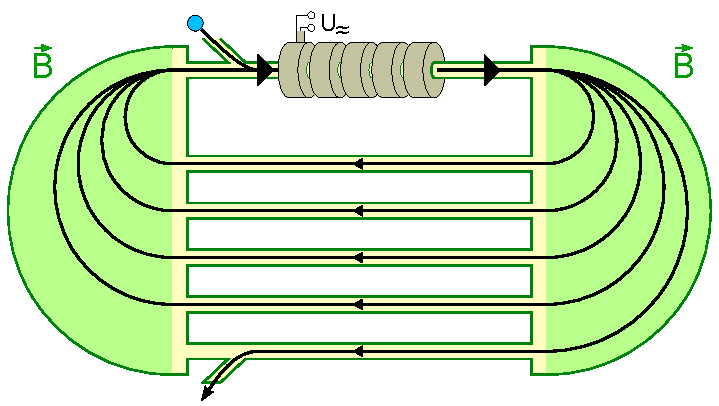
\includegraphics[width = 0.75\textwidth]{ExperimentalSetup/RacetrackMicrotronSketch.pdf}
\caption{Racetrack Microtron. The particles are sent to the linac, and the two deflection magnets make the particles recirculate, until the momenta exceed the capability of the magnetic field.}
\label{fig:RaceTrackSketch}
\end{figure}

A racetrack microtron is characterized by the energy gain per-cycle, $\delta E$, given by the high-frequency electromagnetic field (HF). The energy gain for a single acceleration cavity of the linac is: 

\begin{align*}
\delta E \, = \, e U_{Linac} \cdot cos(\phi)
\end{align*} 

$U_{Linac}$ is the maximum voltage of the linac, and $\phi$ is the phase of the beam relative to the maximum of HF. The beam consist in individual packets (bunches) of electrons, whose rate correspond to the frequency of HF. To be accelerated during each recirculation step, the electron bunches must arrive at entrance of the linac with the correct phase $\phi$. Therefore the electron time of flight per cycle must be an integer or a multiple of the HF period. The time of flight is made of two terms: the first is the time needed to travel in the magnetic field of two $180^{\circ}$ bending magnets, equal to the cyclotron period; the second term is instead given by the straight sections, and remains constant for relativistic motion. 

\begin{equation} \label{eq:TimeofFlight}
T = \dfrac{2 \pi \gamma m_{e} }{qB} + \dfrac{L}{v}
\end{equation}

where $B$ is the magnetic field, $q$ and $m_{e}$ are the charge and mass of the electron, and $L$ is the length of the straight section of the accelerator. The frequency is given by the formula:

\begin{equation} \label{eq:frequency}
f = \dfrac{qB}{2 \pi \gamma m_{e} + \frac{LqB}{v}} 
\end{equation}

From these two equations two conclusion can be drawn:

\begin{itemize}
\item To accelerate slow electrons, with $\gamma = (1,10)$, a magnetic field of $\SI{0.1}{\tesla}$ is used, in order to work with frequencies of ($\SI{2}{\giga \hertz}$,$\SI{4}{\giga \hertz}$), that are easy to control. However with higher energies, and with a small magnetic field, the bending radii is higher and uneconomical.
\item For high energy electrons $\gamma > 10$, to reduce the size of the deflection magnets, it is useful to increase the magnetic field up to $\SI{1}{\tesla}$ of more, with the same band of frequencies $\simeq \SI{}{\giga \hertz}$.
\end{itemize}

This justify the structure of MAMI: a cascade of microtrons to reach progressively higher energies, with the same acceleration frequency at each stage. In MAMI there is a sequence of 4 different microtrons, that are able to accelerate particle up to $\SI{1.6}{\giga \electronvolt}$. 

\begin{figure}[hbtp]
\centering
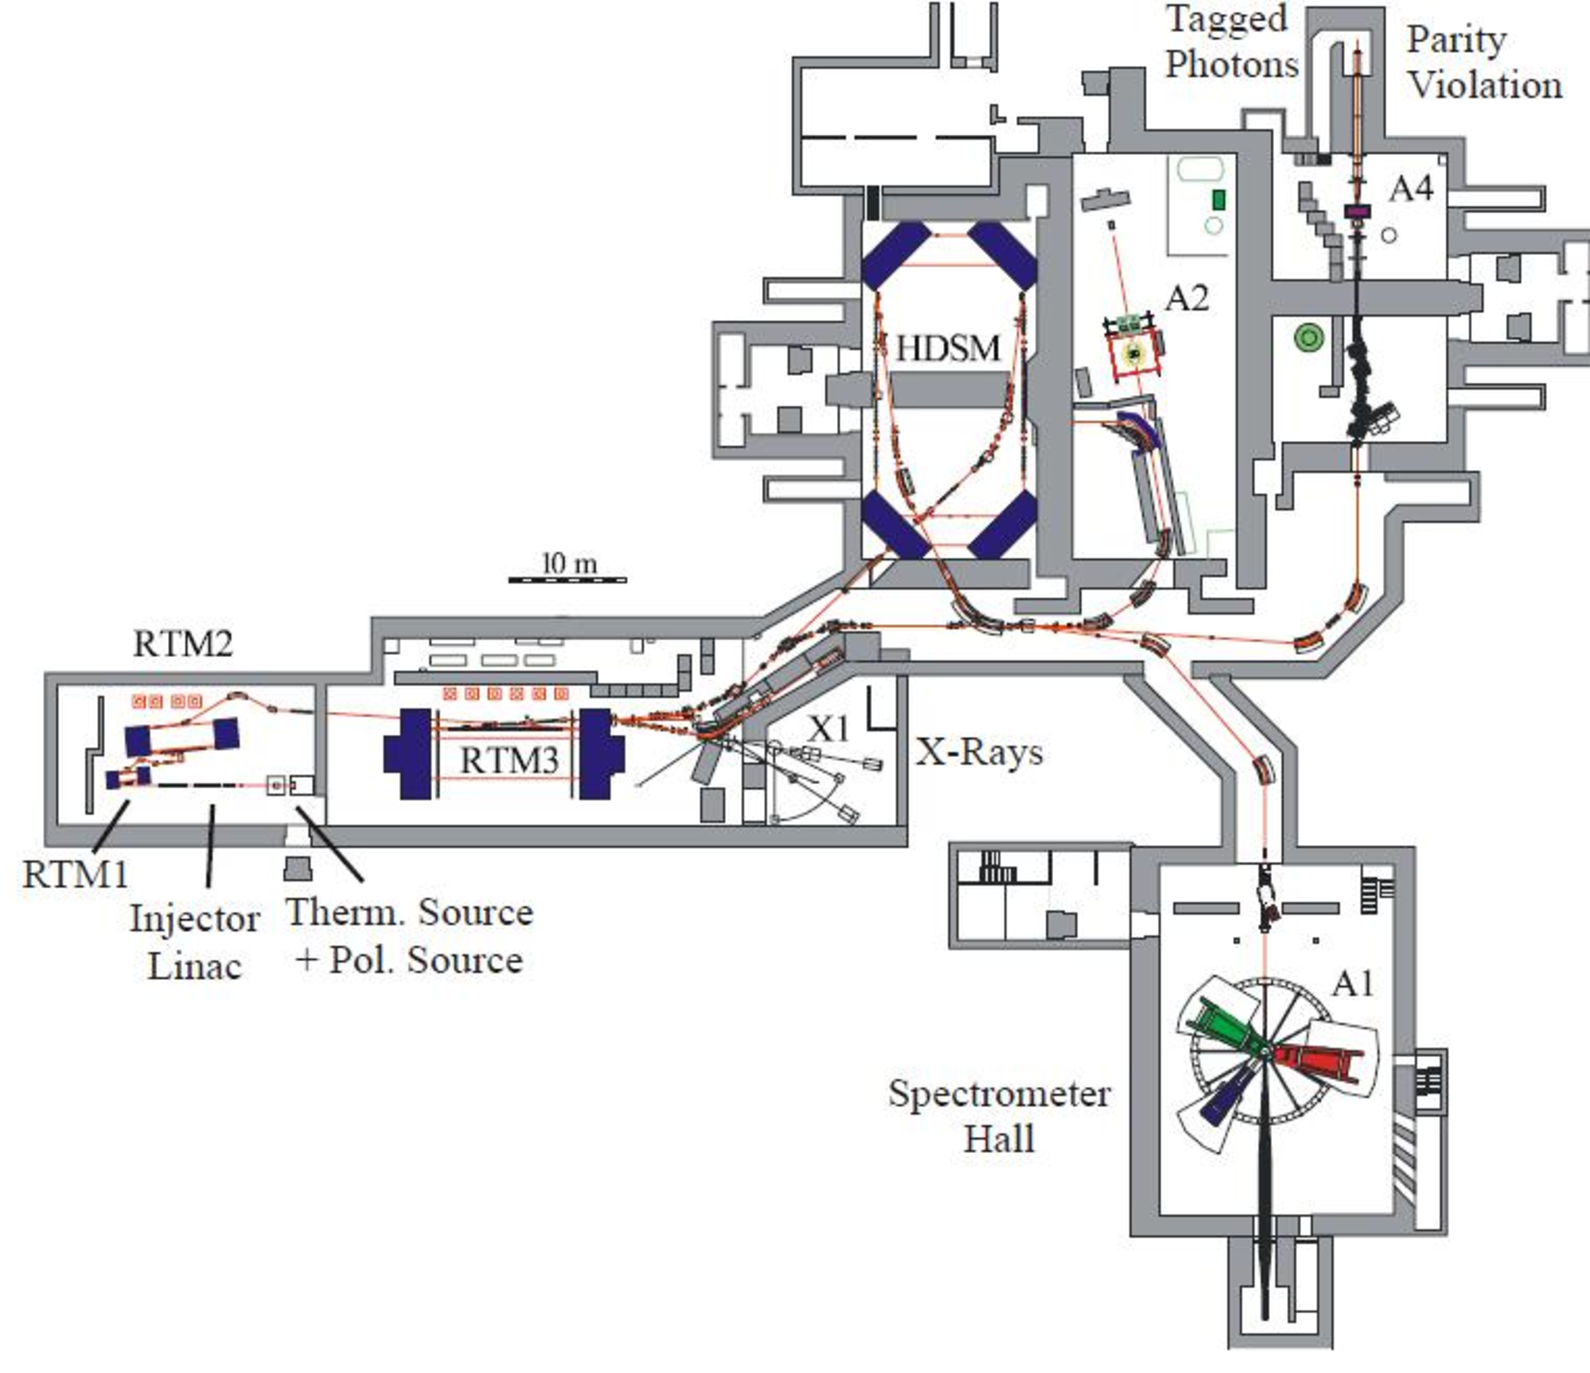
\includegraphics[width = 0.6\textwidth]{ExperimentalSetup/Accelerator.pdf}
\caption{Scheme of the accelerator, with the different experimental halls. A third hall previously used for the A4 experiment, measuring the strange quark content of the proton, is now being used for the novel MESA accelerator and its experiments.}
\label{fig:Accelerator}
\end{figure}

The first stage, shown in figure \ref{fig:Accelerator}, is composed by two small microtrons. The first microtron, RTM1, accelerates the particles up to $\SI{14}{\mega \electronvolt}$ in 18 revolutions. Then the electrons are sent to the RTM2, second microtron that can reach an energy of $\SI{180}{\mega \electronvolt}$. After passing this first stage, the beam is directed towards the RTM3 (race track microtron 3), in the adjacent room, that is large microtron with an end point energy of $\SI{855}{\mega \electronvolt}$. The sequence of RTM1, RTM2 and RTM3 forms MAMI-B, which is operating since 1990-91. A fourth stage, MAMI-C, was built and started operation in 2007. This fourth stage is made by 4 bending magnets, with a bending angle of $90^{\circ}$, and it is designed to achieve energies of $\SI{1.6}{\giga \electronvolt}$. MAMI-C design is different from the other race-track microtrons, and it is not discussed, as it is not necessary for the experiment to reach such high energies.

\begin{figure}[hbtp]
\centering
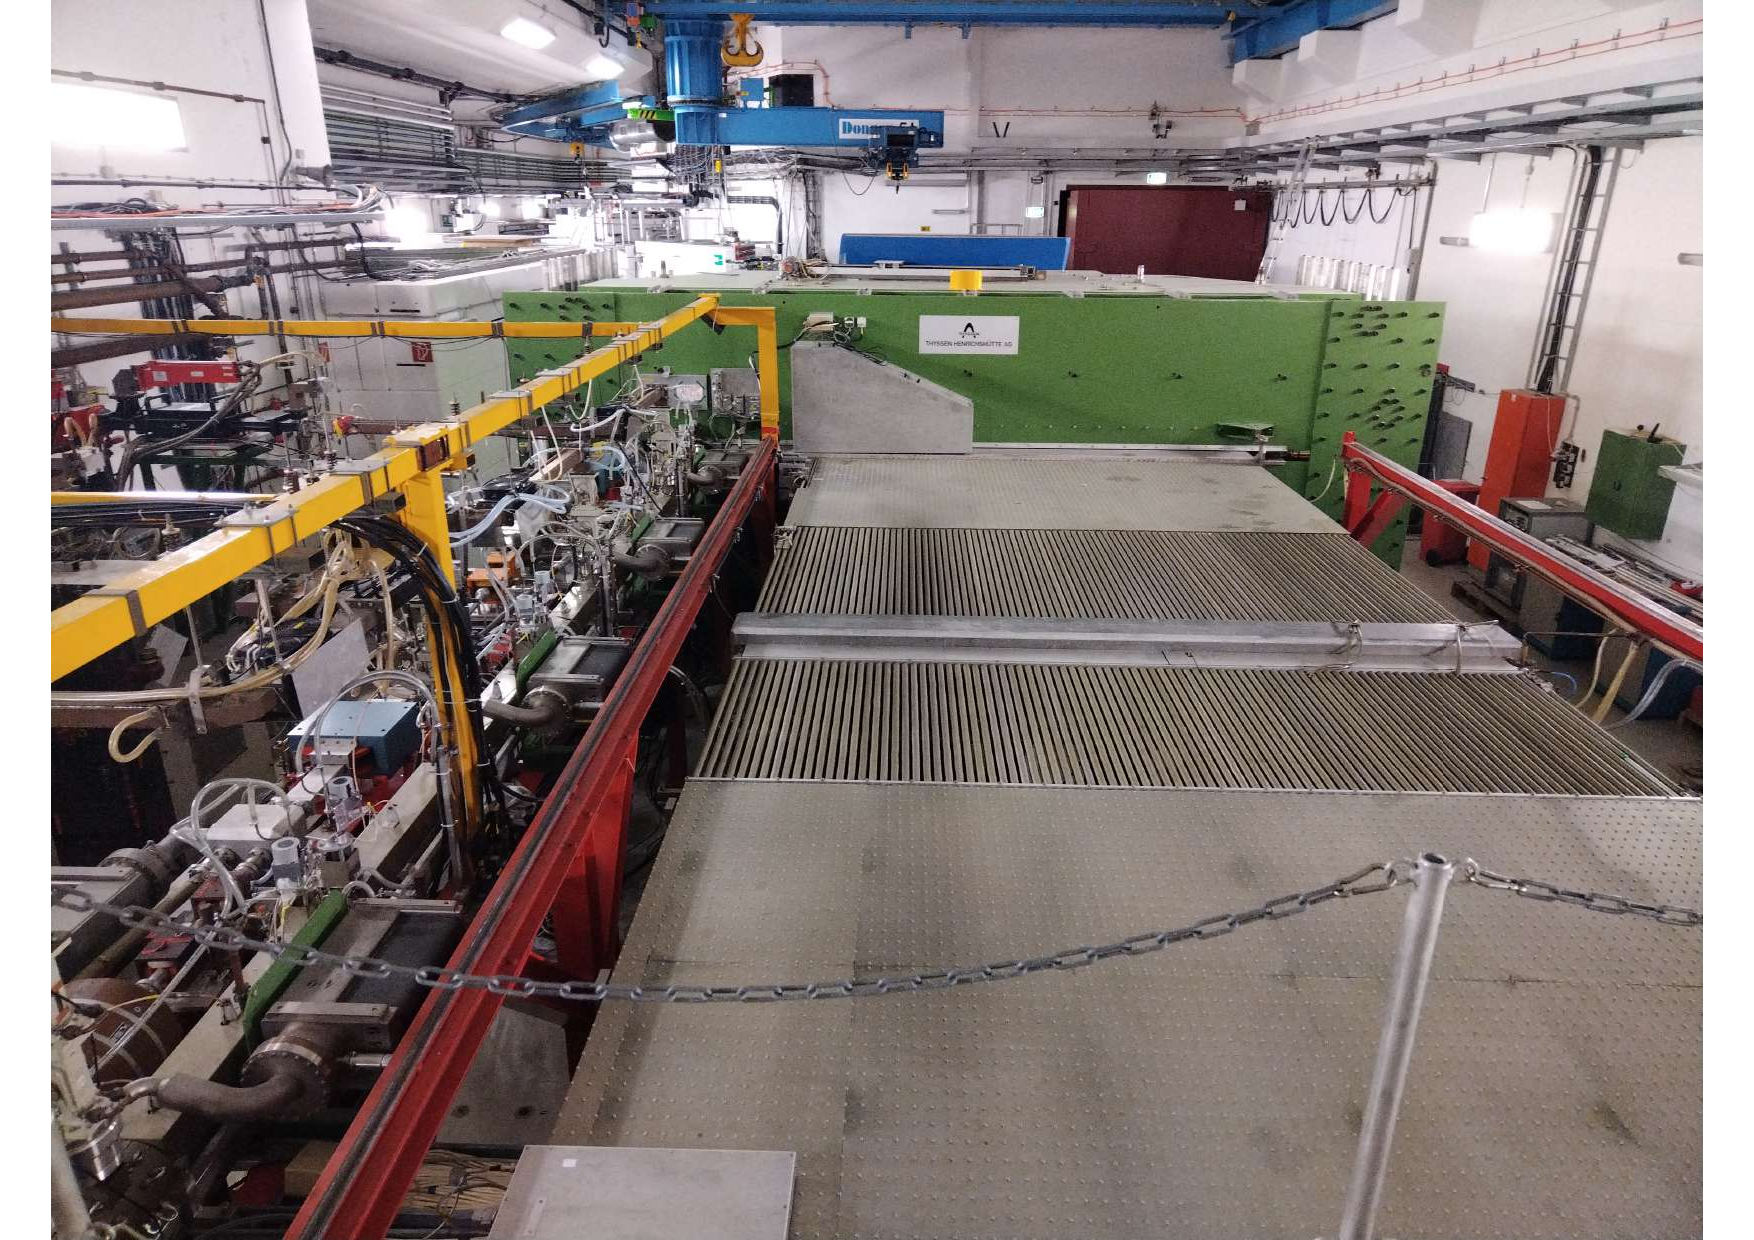
\includegraphics[width=0.75\textwidth]{ExperimentalSetup/Racetrack.pdf}
\caption{Picture of the Racetrack RTM3 in MAMI-B. The Green square at the bottom is one of the deflector magnets, the other one is below the point where the photo was taken. The linac stage is on the left. The tubes at the center of the figure are the paths that the particle cross during the recirculation. The further away from the linac the greater the energy.}
\end{figure}

The operation principles of a microtron is simple to be described. First we consider the gyro-radius for relativist electrons of energy $E$, that is:

\begin{equation}
\qquad r = \dfrac{E \beta}{qcB}
\end{equation}

To have a coherent conditions, we must have that the flight time $\tau = \frac{\lambda}{c}$ of the first recirculation must be an integer multiple of the HF wavelength $\lambda_{HF} = \frac{c}{f_{HF}}$, as shown in equation \ref{eq:frequency}. This means that:

\begin{align*}
\lambda = \tau c =\dfrac{ 2 \pi c r }{\beta c} + \frac{Lc}{v} = \dfrac{2 \pi E}{q B} + L = m \lambda_{HF}
\end{align*}

For the subsequent recirculations, the flight-time at energies $E_{n} = E_{n-1} + \delta E$ must be increased by an integer multiple of HF, too. This lead to a second equation:

\begin{align*}
\dfrac{2 \pi \delta E}{q B} = n \lambda_{HF}
\end{align*}

The minimum gain per cycle is then determined only by the strength of the magnetic field and wavelength $\lambda_{HF}$. The system of these two equations controls the dynamic of the race-track microtrons, and determines the working point of the accelerator.

\subsection{Polarized Beam}

For the beam-normal single spin asymmetry a vertically polarized beam is necessary. At the MAMI electron accelerator it is possible to produce a vertically polarized beam with energy in the range $\SI{180}{\mega \electronvolt} - \SI{855}{\mega \electronvolt}$ \cite{Schlimme:2016rrp}. The procedure to orient the spin vertically is discussed in this section, and the measurement of the degree of polarization is explained. 

The electron source used at MAMI is made by a strained GaAs/GaAsP super-lattice photo-cathode illuminated by circularly polarized light. To alternate the sign of the light polarization, a fast Pockels cell (\cite{Goldstein}) is installed in the optical system of the electron source. The Pockels cell is a wave plate controlled by the electric field, that changes the helicity of the photons impinging on the electrons. A Pockels cell exploits the Pockels effect, that affects crystal with particular characteristics (lack of inversion symmetry). For this type of materials the refractive index is linearly dependent on the applied electric field. By controlling the refractive index, the polarization state of the incident light beam is altered. Since the angular momentum is conserved, the extracted electron carries the same helicity of the incoming photon:
\begin{center}
\begin{equation}
\feynmandiagram [scale = 0.8, transform shape][baseline = (g)]{
	a [particle = \(e^{-}\)] -- [fermion] b  -- [fermion] c [particle = \(e^{-}\)],
	b -- [boson] d [particle = \(\gamma\)],};
\hspace{2cm}
(Jz)_{\gamma} = \pm 1 \qquad (Jz)_{e^{-}} = \mp \frac{1}{2} \rightarrow \pm \frac{1}{2}
\end{equation}
\end{center}

With the fast change of the Pockels cell it is possible to alternate the sign of the polarization. By the insertion of a $\lambda/2$ plate between the laser system and the photo-cathode, the global polarization orientation of the electron beam can be reversed. This is useful because changes directly the sign of the asymmetry measured by the detectors, and allows to identify systematic errors. Usually, two sets of data are taken during an experiment, reversing the orientation of the $\lambda/2$ wave plate. By comparing the results for the two sets of data, the influence of the optical system on the asymmetry measurement is estimated and is used to correct the final result of the asymmetry. However changing the orientation of the $\lambda/2$ requires a certain amount of time and it is usually done for longer beam time. During the experiment described in this thesis, the $\lambda/2$ wave plate orientation was fixed. 

The beam degree of polarization achieved with the electron source is roughly $P = 80 \% $. The degree of polarization reduces the measured asymmetry:

\begin{align*}
A_{measured} = P \cdot A_{n}
\end{align*}

The electrons extracted by the circular polarized laser are longitudinal polarized. A combination of magnetic fields is needed to rotate $\vec{P}$ from longitudinal to transverse orientation. For this purpose two devices are used: Wien filter and a double solenoid, located in the injection beam line, close to the the optical source, as show in figure \ref{fig:Iniezione}

\begin{figure}[hbtp]
\centering
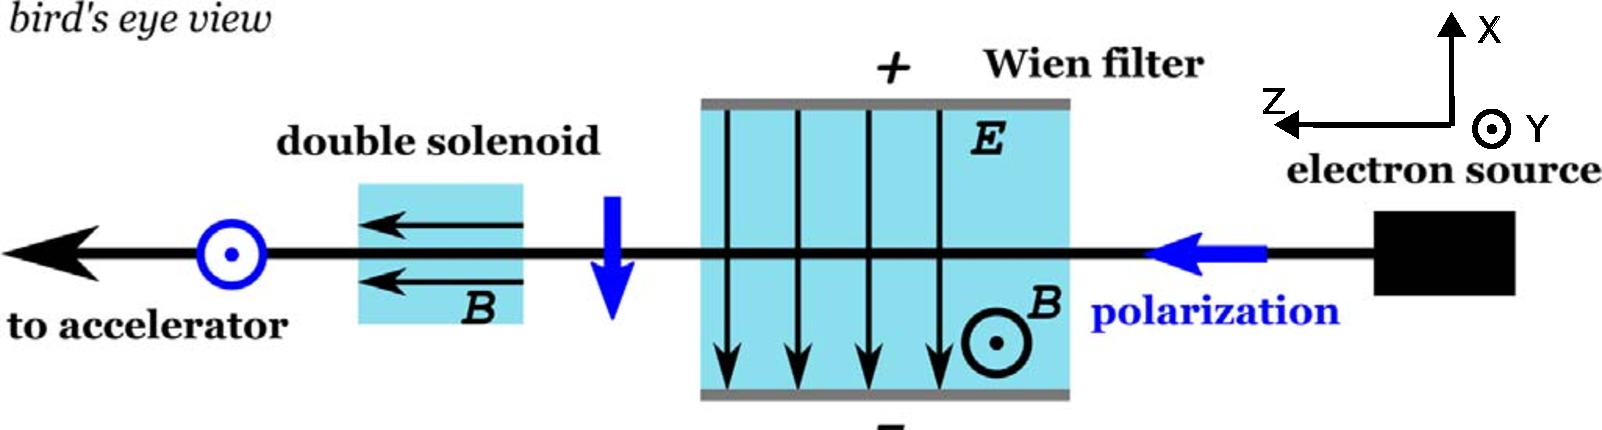
\includegraphics[width = \textwidth]{ExperimentalSetup/InjectionLine.pdf}
\caption{Beam line projection. This figure is taken from the paper \cite{Schlimme:2016rrp}}
\label{fig:Iniezione}
\end{figure}

Looking at the picture, the longitudinal direction corresponds to the $Z$ axis. The $X$ axis is parallel to the second blue arrow, just after the Wien filter, and the $Y$ axis is orthogonal to the page. 
The spin is initially rotated by $90^{\circ}$ in the $X$ direction, with the Wien filter; the subsequent double solenoid aligns the spin to the vertical direction, with another $90^{\circ}$ rotation. 
Once the beam passes the double solenoid, the electrons go through the injector linac, the microtrons and arrive at experimental hall, where the target of the experiments is installed. During the acceleration stage, the spin follows the precession motion, as determined by the BMT equation, due to the various magnetic fields that they encounter during the travel. In our experimental setup, the magnetic field of the various bending magnets that constitute the microtron-cascade are always parallel to the polarization in vertical direction, so the cross product $\vec{B} \times \vec{P} = 0$, and the transverse polarization remains constant. Only the residual horizontal component precedes during the motion. For experiments with longitudinal polarization, after the first spin rotation of the Wien filter and the bending magnets, there is a further rotation determined by the motion of the particles during the acceleration and recirculation in the microtron. Considering this further contribution, the rotation made by the Wien filter is adjusted in such a way that the polarization has the correct alignment in the experimental hall. The rotation angles due to the various magnetic field are known from simulations and also directly measured for some energies: for a beam of $\SI{570}{\mega \electronvolt}$ the rotation angle is $\ang{55}$ with an accuracy of $\pm \ang{2}$. In our case, this further rotation has only a small effects on the residual horizontal component. This horizontal component is accurately minimized by MAMI operators at the beginning of the beam time, and its effects on the measurement are negligible. 

MAMI was not developed for experiments with transverse polarization, so it is not possible to measure directly the transverse component. However the vertical polarization is deduced from the determination of the total beam polarization and the residual horizontal components. For this purpose a M\o ller , Compton and Mott polarimeters are used.

\subsection{Vertical Polarization Measurement}
Three polarimeters are installed in MAMI: a Mott, M\o ller and A Compton polarimeter. The Compton and Mott polarimeters are located before the injector linear accelerator (see figure \ref{fig:Accelerator}), close to the beam source, where the \SI{3.5}{\mega \electronvolt} electrons have gone through the Wien filter and the double solenoid. The M\o ller polarimeter, instead, is installed in the spectrometer hall, where the beam is delivered. The M\o ller polarimeter is sensitive to the longitudinal component of the polarization, while the Mott and Compton polarimeter are sensitive to the $Z$ and $X$ component. 
When the beam is polarized longitudinally, the total polarization is measured by the M\o ller polarimeter, in the spectrometers hall. The procedure for the polarization alignment is the following: at the beginning of the beam time the Mott polarimeter measures $P_{z}$ for different settings of the double solenoid field, fixing the rotation angle of the Wien filter nominally at $\ang{90}$. Changing the double solenoid filed, the horizontal polarization component ($P_{x}$) is minimized. A second minimization follows, using the M\o ller polarimeter and changing Wien filter rotation angles, leaving the double solenoid field fixed. In this way also the longitudinal component $P_{z}$ is minimized. With the new Wien filter setting, another measurement is performed with the Mott polarimeter. With this procedure, the $P_{x}$ and $P_{z}$ components are completely minimized, and the beam polarization is parallel to the $Y$ axis, in the end.
At this point, the polarization is correctly aligned, and the experiments can start. The last polarimeter, the Compton, is not to obtain the vertical polarization, but can measure the variation of the degree of polarization during time, as explained is \cite{Schlimme:2016rrp} 

In the last measurement of $A_{n}$ at MAMI \cite{Esser:2018vdp} the Moller and Mott polarimeters were available. In this way, it is also possible to estimate the systematic uncertainty for the degree of polarization, which is the relevant contribution of the systematic uncertainty for the measurement of $A_{n}$. The value of systematic error for the previous experiment is about $1 \, ppm$. For the experiment described in this thesis, the polarization was aligned to the transverse direction using only the Mott polarimeter, obtaining $P = 0.79\%$. The M\o ller polarimeter was not available, and we could not estimate the systematic uncertainty of the degree of polarization.

\subsection{Mott Polarimeter}

In this section we describe the theory of the Mott polarimeter. The Mott polarimeter exploits the asymmetry in the cross section due to the spin dependence. From the asymmetry we can measure the polarization of the beam. 
Let's suppose that we have an electron beam that is sent towards a nucleus of charge $Ze$. We know from theory \cite{MottElectron} that the spin of the incident electron interacts with the electromagnetic field produced by the nucleus.
The magnetic field seen by a particle with speed $\vec{v}$ near a nucleus is:

\begin{align*}
\vec{B}_{nucleus} = \frac{-\vec{v} \times \vec{E}_{nucleus}}{c}  = \frac{Ze}{mc r^{3}} \vec{L} 
\end{align*}

This magnetic field is coupled with the magnetic momenta of the electron $\mu_{e}$.

\begin{equation}
V = - \vec{\mu} \cdot \vec{B}_{nucleus} = \frac{Ze}{mcr^{3}} \vec{L} \cdot \vec{S}_{e^{-}}
\end{equation}

The second equation represents the spin-orbit interaction potential. This term yields the polarization dependence of the cross section. Let's consider an incident particle that scatters from a nucleus at an angle $\theta$, as shown in the figure:

\begin{figure}[hbtp]
\centering
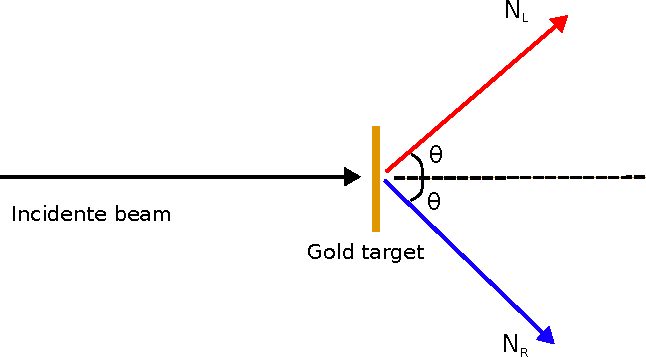
\includegraphics[width = 0.45\textwidth]{ExperimentalSetup/MottScattering.pdf}
\caption{Scheme of the Mott scattering, the polarization is orthogonal to the plane,  $ \vec{n} = \frac{\vec{k} \times \vec{k'}}{|\vec{k} \times \vec{k'}|}$. The red and blue arrows represent two scattering events with the same $\theta$, but opposite $\vec{n}$}
\label{fig:MottScatt}
\end{figure}

The cross section can be modeled highlighting the dependencies on the polarization $\vec{P}$:

\begin{equation} \label{eq:MottCross}
\dfrac{\partial\sigma(\theta)}{\partial \Omega} = I(\theta) [1 + S(\theta) \vec{P} \cdot \vec{n} ]
\end{equation}

In the equation above, the cross section is divided in two terms: $I(\theta)$ represents the term that does not depend on the polarization, while the second term contains the dependence on the polarization, through is the Sherman function $S(\theta)$; also called the asymmetry function \cite{MottElectron}. The unit vector $\vec{n}$ is normal to the scattering plane, and it is defined as:

\begin{align*}
\vec{n} = \dfrac{k \times k'}{|k \times k'|}
\end{align*}

Where $k$ and $k'$ are the wave vectors associated with the incident and scattered electrons. The direction of $\vec{n}$ is parallel to the angular momentum $L$, and depends on whether scattering is to the left or to the right.
Let's suppose our initial beam has a polarization $P$, that can also be expressed as:

\begin{align*}
P = \frac{N_{\uparrow} - N_{\downarrow}}{N_{\uparrow} + N_{\downarrow}}
\end{align*}

Where $N_{\uparrow}$ and $N_{\downarrow}$ are the number of electrons with spin up and spin down. The Mott polarimeter measures the number $N$ of scattered electrons at a fixed angle $\theta$, in the two directions right and left (figure \ref{fig:MottScatt}). Using the equation (\ref{eq:MottCross}), the scattered electrons to the left side $N_{L}$ and to the right side $N_{R}$ are equal to: 

\begin{align*}
N_{L} &= N_{\downarrow}[1 + S(\theta)] + N_{\uparrow}[1 - S(\theta)] \\
N_{R} &= N_{\uparrow}[1 + S(\theta)] + N_{\downarrow}[1 - S(\theta)]
\end{align*}

The asymmetry $A(\theta)$ of the scattered electron between left ($N_{L}$) and right ($N_{R}$) is given by:

\begin{align*}
A(\theta) = \frac{N_{L} - N_{R}}{N_{L} + N_{R}} &= \dfrac{N_{\downarrow}(1 + S(\theta)) + N_{\uparrow}(1 - S(\theta)) - N_{\uparrow}(1 + S(\theta)) - N_{\downarrow}(1 - S(\theta))}{N_{L} + N_{R}} = \\ 
&= \dfrac{(N_{\uparrow} - N_{\downarrow})}{(N_{\uparrow} + N_{\downarrow})}S(\theta) =  P \cdot S(\theta)
\end{align*}

The last step of the equation gives the beam polarization in terms of $A(\theta)$, the asymmetry measured by the Mott polarimeter, and the function $S(\theta)$, the Sherman function. The Mott polarimeter in MAMI, installed after the double solenoid, measures the scattering asymmetry $A(\theta)$ for electrons of $\SI{3.5}{\mega \electronvolt}$ with a thin gold target.  

\section{Experimental Hall Setup} \label{ExperimentalHall}

MAMI experimental halls are named with the capital letter A followed with a number. In A2, for example, photo-nuclear reactions are studied to investigate the fundamental physics at the scale of nuclear dimensions. The experimental hall where the experiment described in this thesis is conducted is the A1 hall. We will describe briefly the main operating detectors that are installed and the details that are interesting for the transverse asymmetry measurement.
In the A1 hall the beam is delivered with energy in a range starting from $\SI{180}{\mega \electronvolt}$ up to $\SI{1.6}{\giga \electronvolt}$. Energy greater than $\SI{855}{\mega \electronvolt}$ are reached with the last acceleration stage HDSM, shown in figure \ref{fig:Accelerator}. Because the electron energy of our experiment is $\SI{570}{\mega \electronvolt}$, the beam passes only through the first acceleration steps, and is extracted from the RTM3 and directly sent to the A1 experimental hall, without going through the HSDM stage. 

\begin{figure}[!h]
\centering
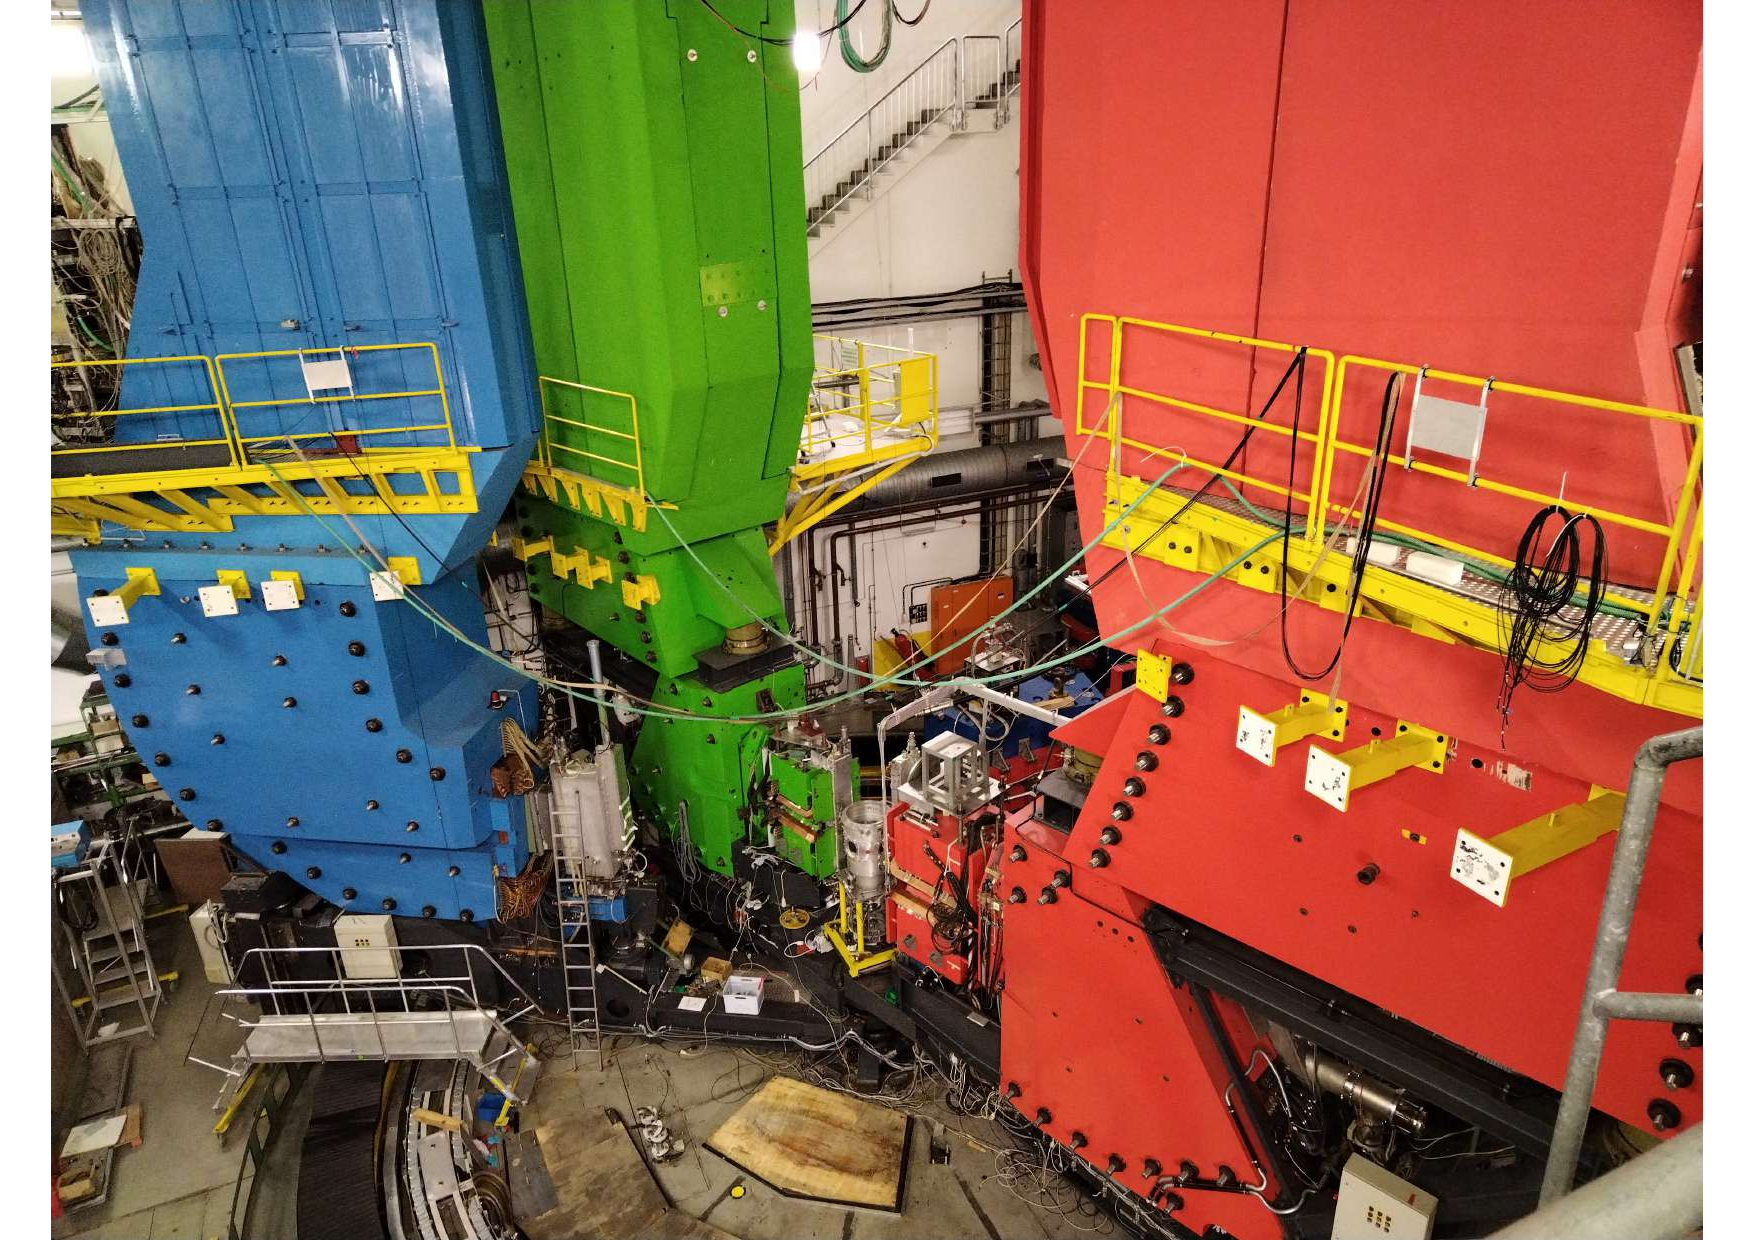
\includegraphics[width = 0.9\textwidth]{figures/twoSpektrometer.pdf}
\caption{Picture of the A1 spectrometers hall, the spectrometers red and blue are used during this experiment. At the center of the picture is possible to observe the scattering chamber.}
\label{fig:TwoSpektr}
\end{figure}

Inside the A1 hall three large magnetic spectrometers are placed on a circular rail-track around the target chamber (figure \ref{fig:TwoSpektr}). They where designed and built in $1993$ to perform high precision measurement of electron scattering in coincidence with other hadron detection, with high resolution in the determination of the particle momenta $\frac{\delta p}{p} < 10^{-4}$. The spectrometers develop vertically with a height of $\SI{15}{\meter}$, and the scattered electrons and the other particles are deflected with respect to the scattering plane with the use of magnetic fields. The figure \ref{fig:TwoDetectors} shows the path of the particles scattered from the target. The spectrometers used for the transverse asymmetry measurement are the red and blue ones. There are multiple reasons why the particle are deflected in the vertical direction, that can be summarized in two points: 

\begin{itemize}
\item reason of space: a horizontal setup would not fit in the dimension of the building; in addition this would not allow to rotate the spectrometers by a variety of angles
\item reduce background and noise: in fact the high beam intensity at MAMI is a source of noise and background events which can be reduced by detecting the scattered particles away from the beam direction.
\end{itemize}    

\begin{SCfigure}[30][!ht]
\centering
\caption{Image of the spectrometers of A1 hall. The spectrometers can be rotated using a system of rail-tracks that are visible at the bottom of the image. The electrons are scattered and then deflected in the vertical direction by the magnetic field (green lines). This picture is taken from behind the target. The target is roughly at the center of the image where the two green lines join. The electron are coming from the opposite direction, with respect to the spectrometers.}\label{fig:TwoDetectors}
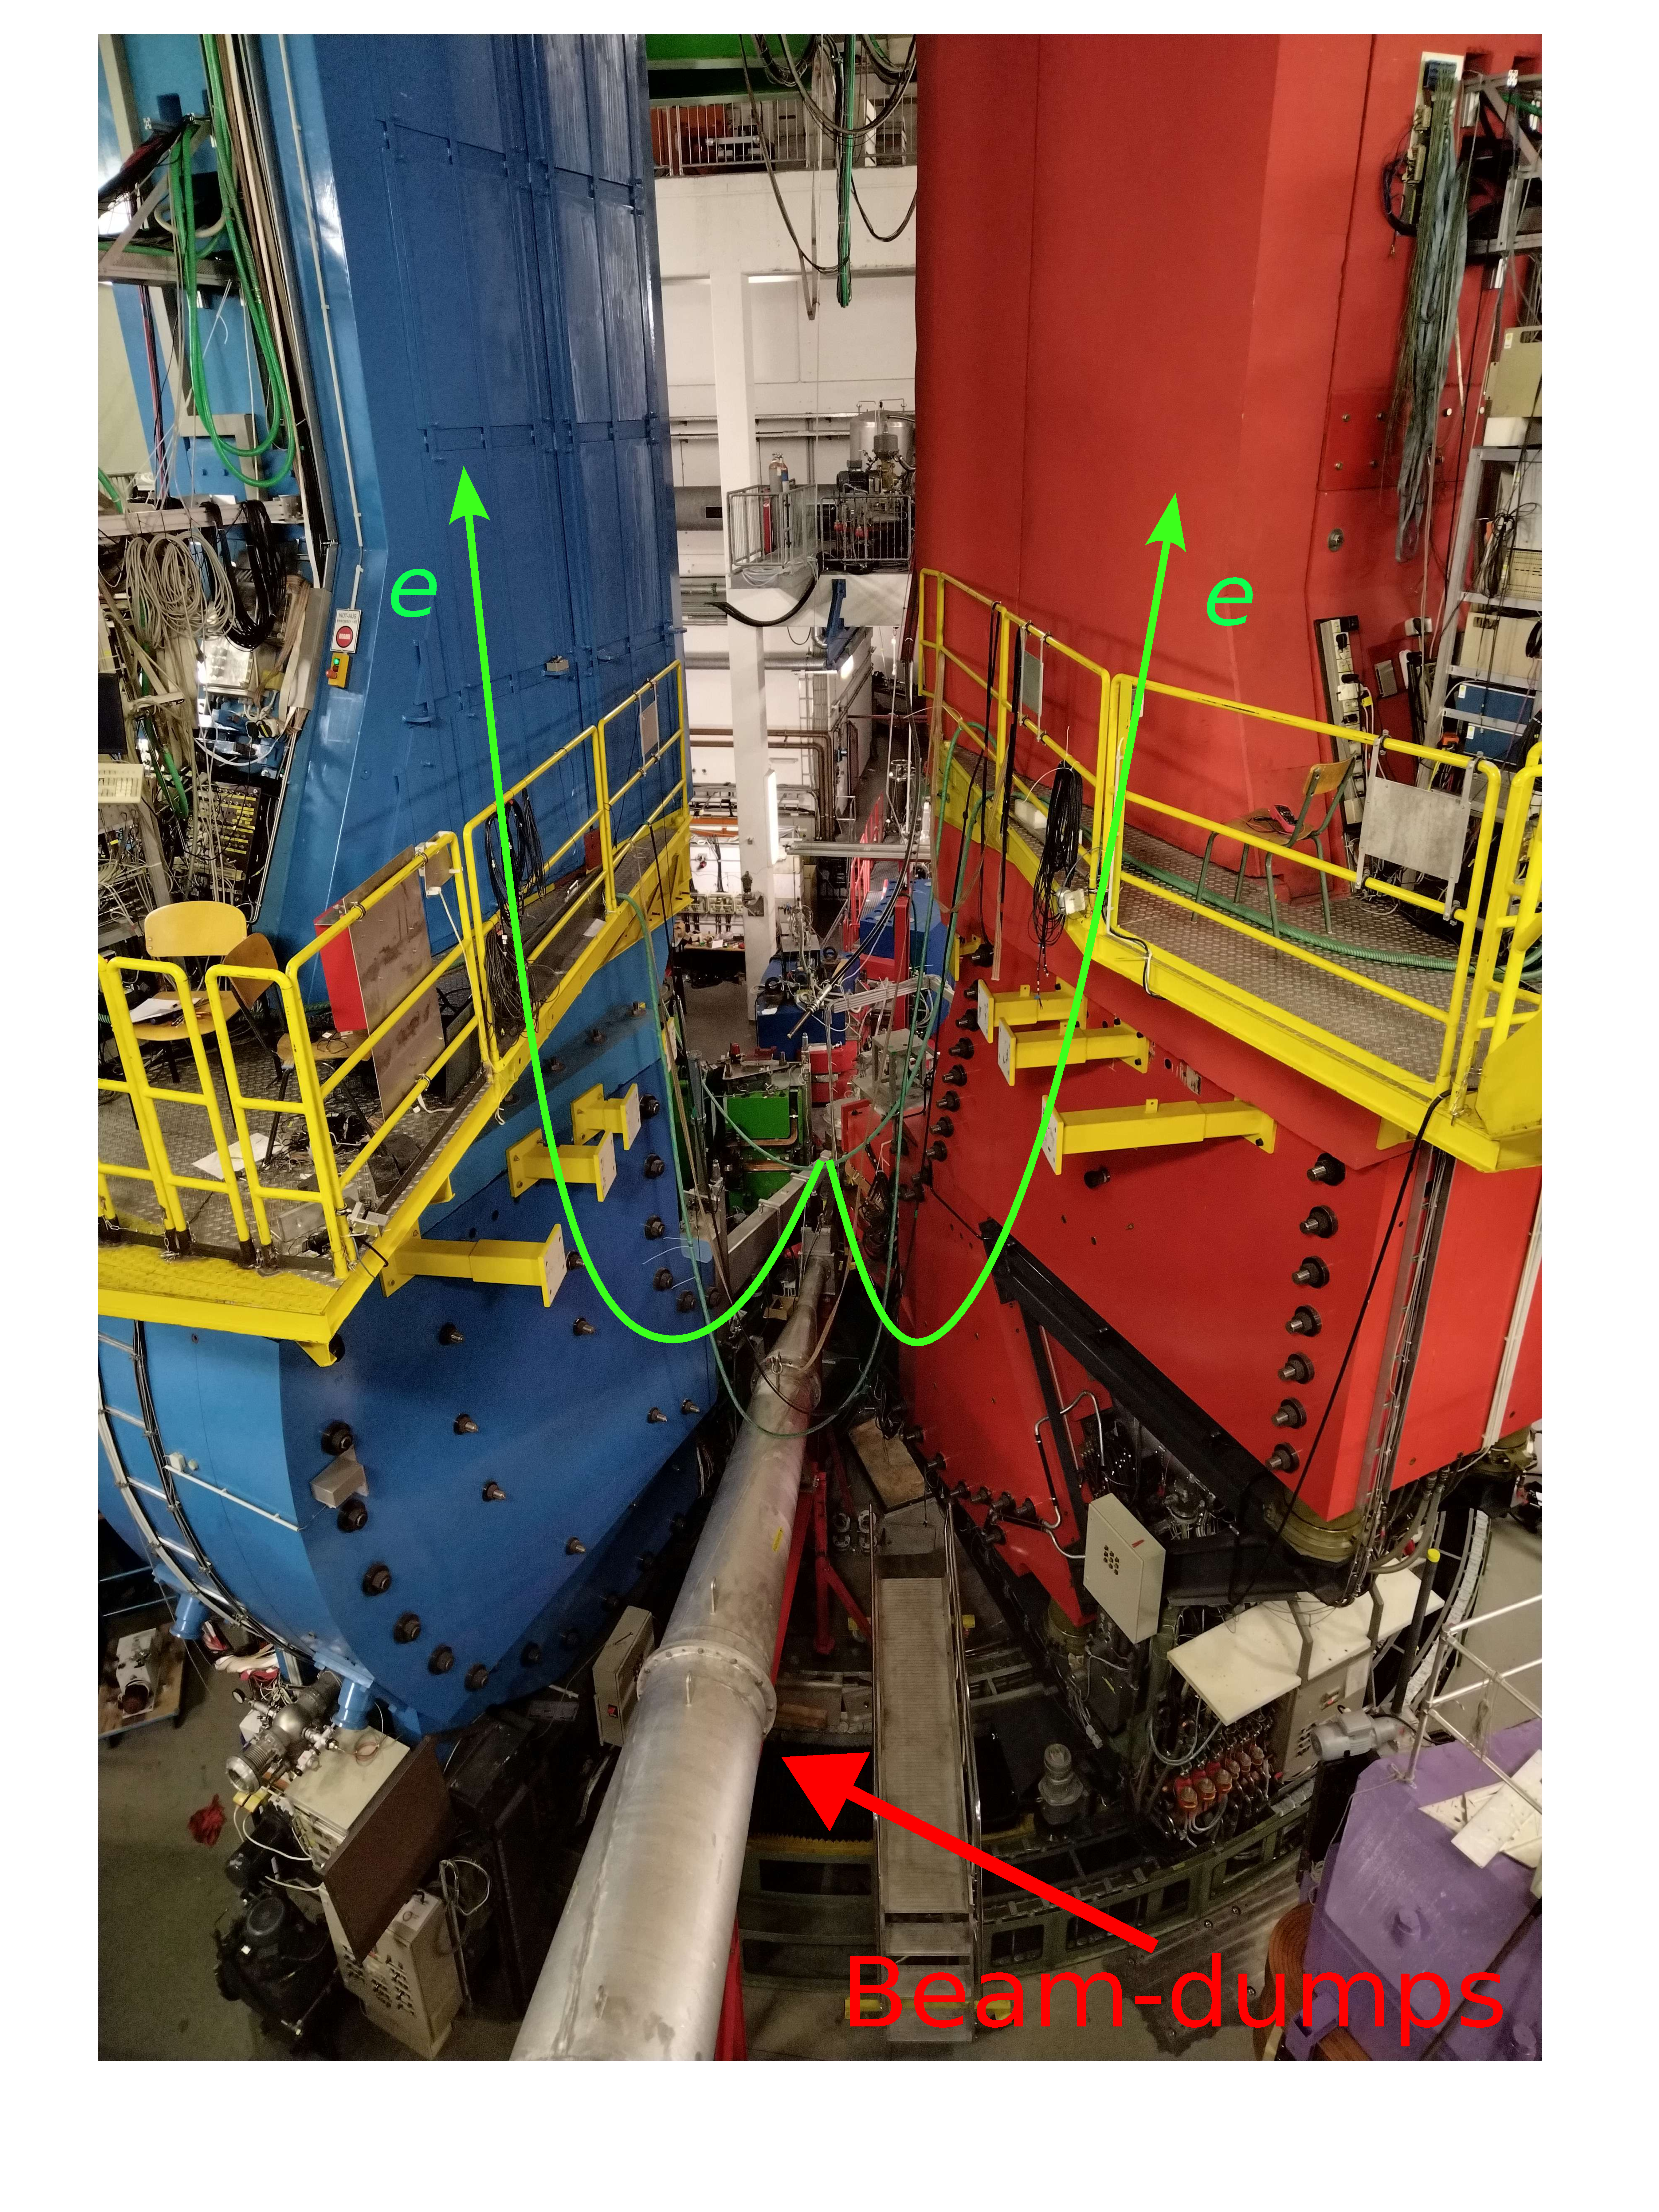
\includegraphics[width = 0.5\textwidth]{ExperimentalSetup/A1_Dietro.pdf}
\end{SCfigure}
  
Once a particle is scattered in the acceptance region of the spectrometers, it is deflected by the magnetic field and passes through the drift chamber, which occupies the first third in height of the spectrometers. 
When the particle is at the height of the platform in the figure \ref{fig:TwoDetectors}, it impinges on a layer of plastic scintillator, and after that a Cherenkov detector  measures the particle speed $v$. In figure \ref{fig:internal} the spectrometer A internal, taken during the installation of detector A, is shown. The determination of both the particle speed $v$ and momenta (drift chamber) allows particle identification.
\begin{SCfigure}[30][!h]
\centering
\caption{Internal of the spectrometer. This image was taken during the installation of the detector A inside the red spectrometer, that is accessible from the platforms visible in the picture \ref{fig:TwoDetectors}}
\includegraphics[width=0.30\textwidth]{ExperimentalSetup/Detectors/position.pdf}
\label{fig:internal}
\end{SCfigure} 

Despite the possibilities offered by the already existing setup, for the beam time of interest none of these components was used directly in the estimation of $A_{n}$. The reason is due to the high intensity of the beam that is used in the experiment, which is far from the optimal operating conditions of the components, that are suited for rates lower than the ones expected for beam normal single spin measurements. The spectrometers are used indirectly, for the alignment of scattered electrons to our detection system.


\section{Detector Description} \label{detectors}
In this section we will describe the electronics and the detectors used to measure the transverse spin asymmetry.
For this experiment we are going to measure the transverse asymmetry at one fixed angle, corresponding to a transferred momentum of $Q = \SI{0.2}{\giga \electronvolt}$. The electrons detection is 
made via two thin blocks of fused-silica that are coupled to PMTs. When a scattered electron hits the fused-silica (refractive index $n = 1.45$) Cherenkov light is emitted. The emitted Cherenkov light can extract one electron in the photocathode, which will be amplified by the PMT dynode structure. This sequence of event triggers the PMT and produce an output signal.

In the experiment two detectors are installed and read-out independently. The detector A is placed at an angle of $+\theta$, while detector B is placed at $-\theta$. We expect to measure the same absolute value of the transverse asymmetry, with an opposite sign due to the different orientation. 
The two detector are made by 3 PMTs and 8 PMTs coupled with two blocks of fused-silica, as shown in \ref{fig:DetectorAB}.

\begin{figure}[hbtp]
\centering
\subfloat[][\emph{Detector B}]{
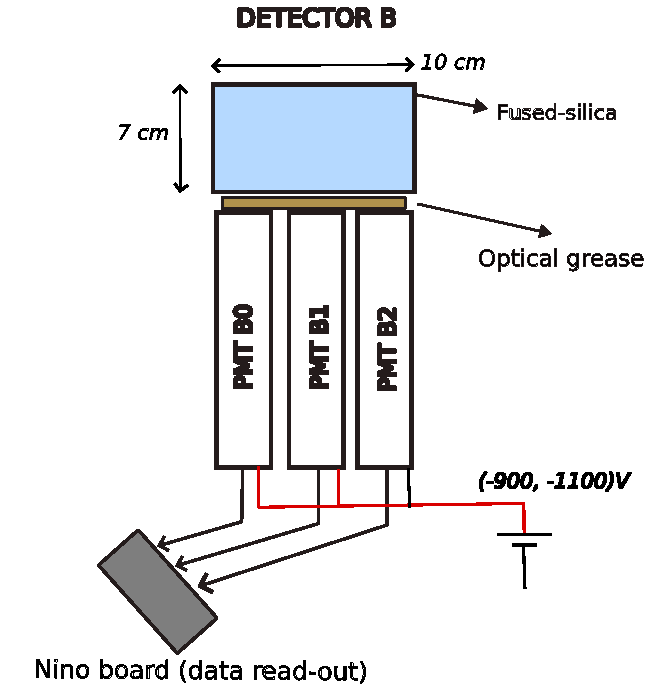
\includegraphics[width = 0.40\textwidth ]{ExperimentalSetup/Detectors/DetectorB.pdf}}
\subfloat[][\emph{Detector A}]{
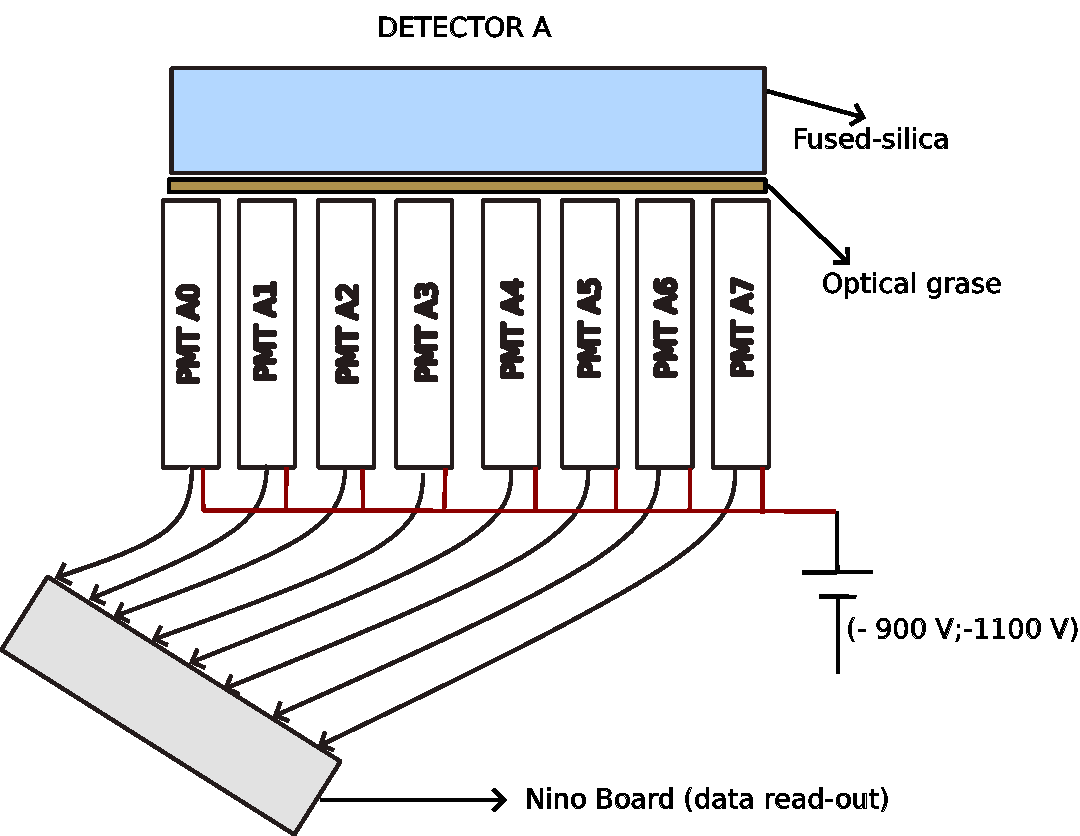
\includegraphics[width = 0.55\textwidth ]{ExperimentalSetup/Detectors/detectorA.pdf}}
\caption{Detector A and B scheme. Each PMT is coupled to the same fused silica bar. The PMTs located at the edges of the fused-silica bars are expected to measure lower rates with respect to the PMTs located near the center. The output signals have negative voltage and are read out by the NINO board.}
\label{fig:DetectorAB}
\end{figure}

These two detectors are placed inside the spectrometers presented in \ref{fig:TwoDetectors}, between the top of the drift-chamber, which occupies the first third in height of the spectrometer, and just below the panel of scintillator. During the experiment, the drift chamber of the spectrometers is turn off, and also the PMTs coupled to the spectrometer scintillators are not powered.
As mentioned above, the scattered electron are deflected in the vertical direction by the magnetic field of the spectrometer. It is important to mention the differences between the new and the old electronic setup. In the old electronic setup the output signal of the PMTs was integrated during the time interval of each sub-event, and therefore the single scattered electron could not be counted. The advantage of this method is that the electronics is simpler. However, this old method is affected by a baseline noise and it is not good for the future experiments with lead target, where the expected rates are lower than the rates on carbon.
With the new electronics, the single electrons are counted, and this will enable the future measurements with lead, improving the accuracy. 

\begin{figure}[hbtp]
\centering
\subfloat[][\emph{Detector B}]
	{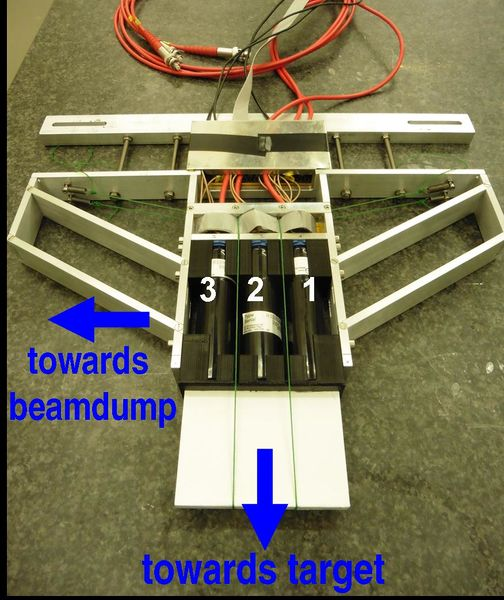
\includegraphics[width = 0.35\textwidth]{figures/504px-Blackfalcon.jpg}} \quad
\subfloat[][\emph{Detector A}]
	{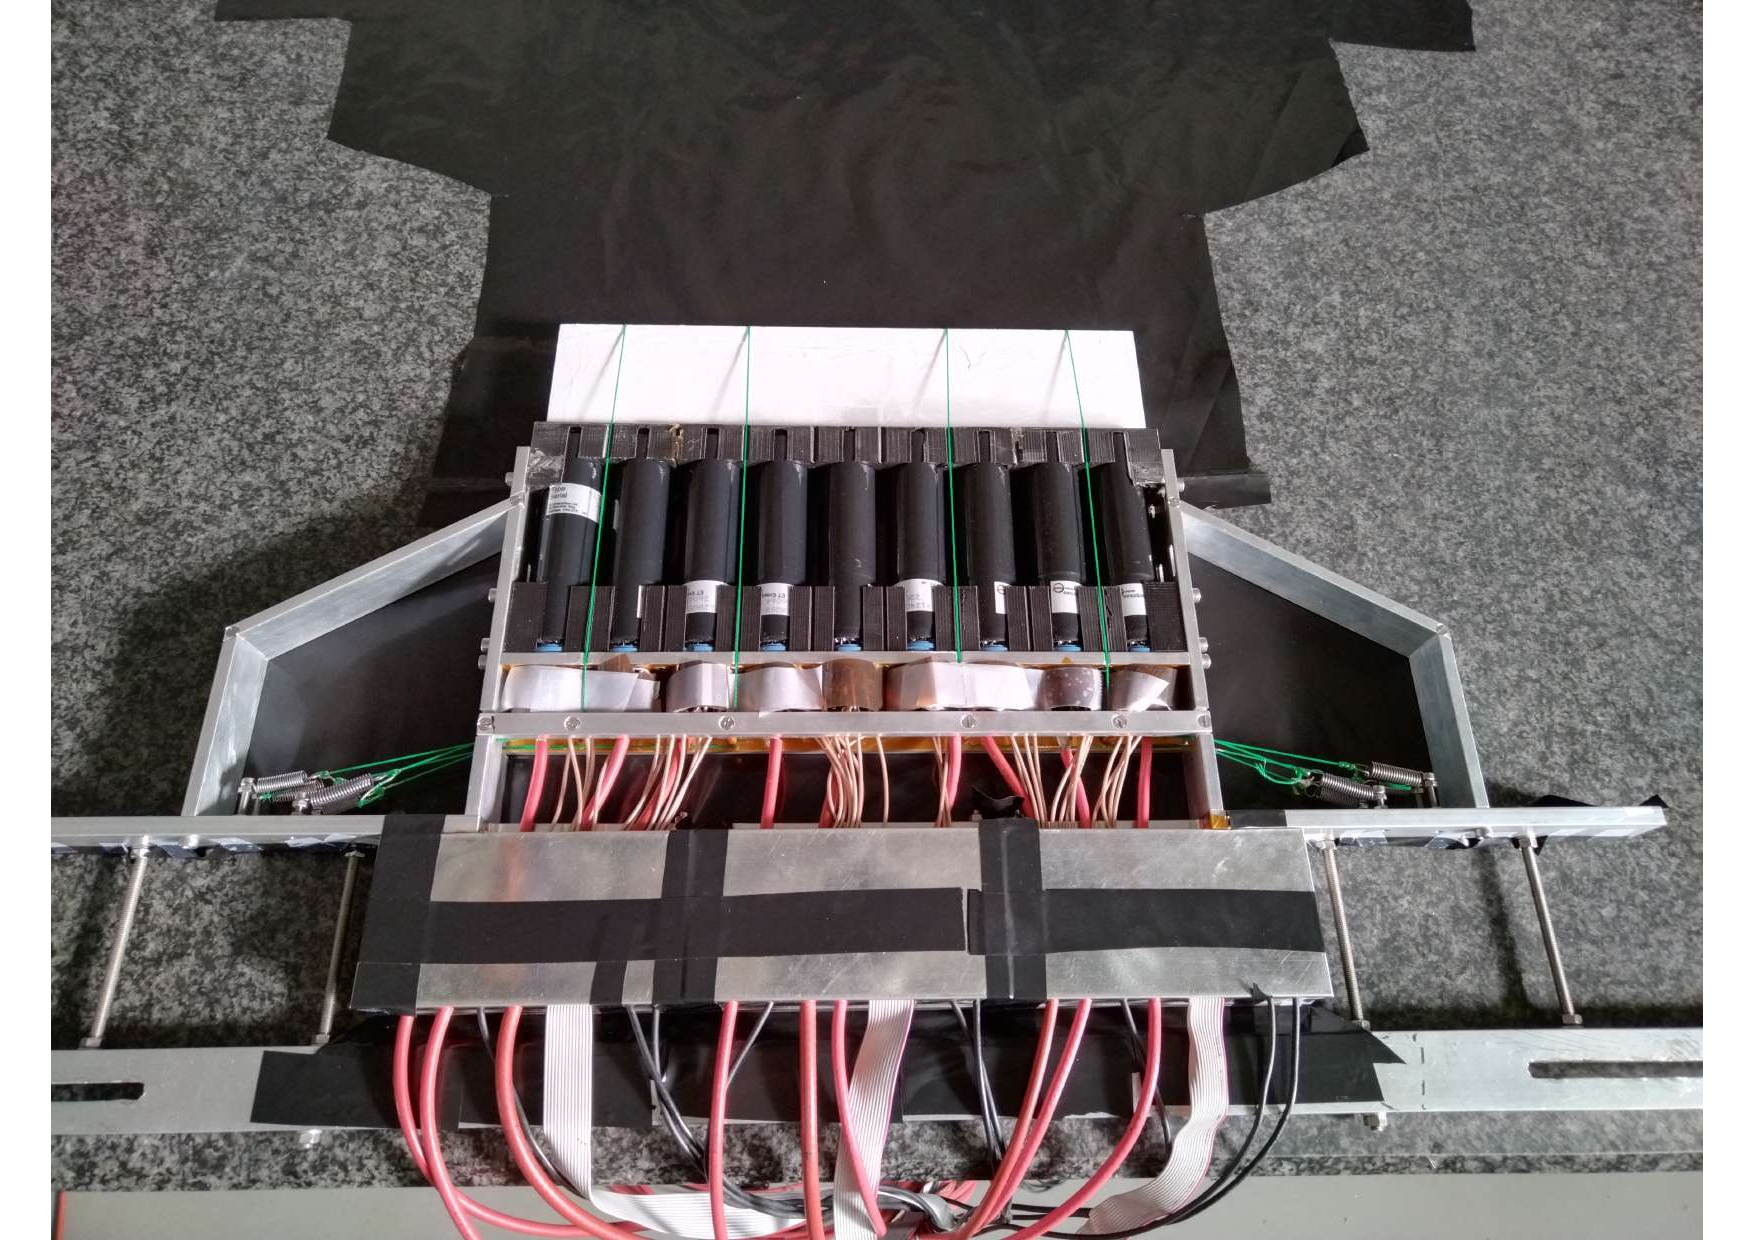
\includegraphics[width = 0.45\textwidth]{figures/IMG_20221110_122246.pdf}} \quad
	\label{fig:Detectors}
\caption{Picture of the two detector taken in the clean room. The white blocks are the fused silica bars that produces the Cherenkov light, the cylinders below are the PMTs, triggered by the passage of the particle. }
\end{figure}

Here we report the characteristic of the two detector that are relevant for the data analysis: 

\begin{itemize}
\item detector B size: $\SI{7}{\centi \meter} \times \SI{10}{\centi \meter} \times \SI{1}{\centi \meter}$
\item detector A size: $\SI{7}{\centi \meter} \times \SI{30}{\centi \meter} \times \SI{1}{\centi \meter}$
\item Number of dynodes of the PMT: 12
\item The Power voltage for the PMT in negative, in the range of ($\SI{-900}{\volt}$, $\SI{-1100}{\volt}$)
\item refraction index $n$ of the fused-silica is $1.45$.
\item maximum gain of $22 \cdot 10^{6}$.
\end{itemize}

The PMTs are coupled to the fused-silica with an optical grease suited for ultraviolet light. The PMTs positioned at the center of the fused-silica bar have an effective area coverage larger than the PMTs at the edge and their rates are expected to be higher compared with the other PMTs. 

\section{Beam Monitors}

In MAMI, several monitors are placed along the beam line to check the beam quality and measure parameters such as current intensity, energy and relative position of the beam. This section summarizes the operating principles of the monitors installed at MAMI. Some details will be given in the appendix, for a complete discussion please refer to the following paper \cite{M_Dehn}.
The monitors available at MAMI are constituted by resonant cavities. With the resonant cavities it is possible to measure the various quantities, with the underlying physical principle that the passage of charged particles through these cavities excites some electromagnetic resonant modes\footnote{TM mode, where the magnetic field is completely transverse respect to particle momenta} (see figure \ref{fig:CylindricMonit}) which can be detected and analyzed by an analog circuit, and related the beam parameters.

\begin{figure}[!hbtp]
\centering
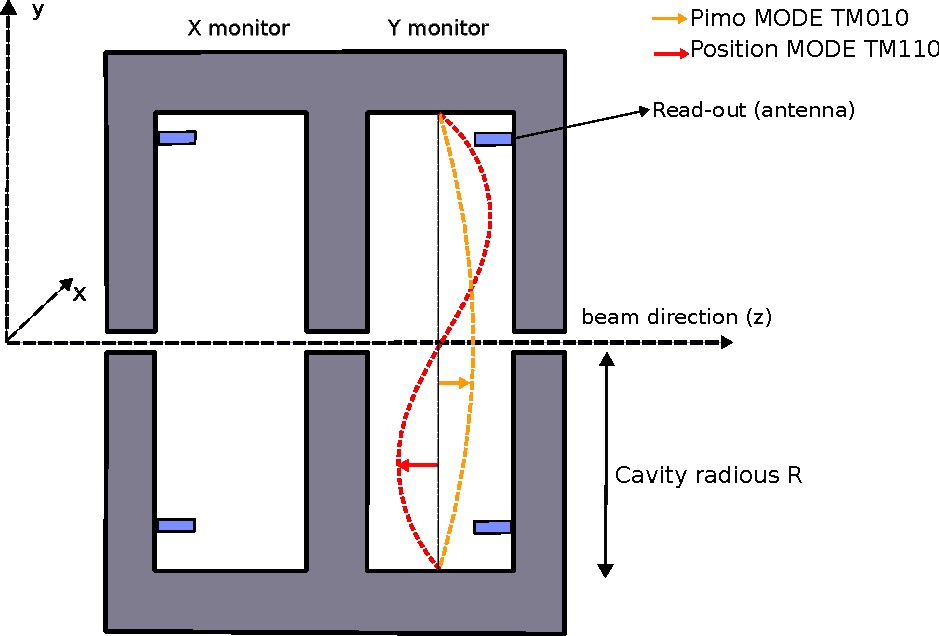
\includegraphics[width = 0.65 \textwidth]{ExperimentalSetup/Monitors.pdf}
\caption{Scheme of the Cylindrical cavities installed at MAMI. In red we have the $TM_{110}$ mode, used to measure the position of the beam, in yellow the $TM_{010}$ mode, to measure the intensity of the beam.}
\label{fig:CylindricMonit}
\end{figure}


Before going into the details, it is necessary to define some quantities that will be used later in the discussion. We define the Shunt-impedance $r_{s}$ as:

\begin{equation}
r_{s} = \frac{|V_{\|}|^{2}}{P}
\end{equation}

Where $P$ is the power absorbed by the cavity when a particle excites one of the resonant mode, and $V_{\|}$ is defined as the effective voltage experienced by a charged particle along a straight line, which can be computed as:

\begin{align*}
V_{\|} = \frac{1}{q}  \int_{s_{0}}^{s^{1}} \vec{E}_{s} \cdot  \,d \vec{s}
\end{align*}

The Shunt impedance is a measure of the interaction strength between a cavity and a charged particle, and can also be expressed using the $Q$ value of the cavity, the maximum energy stored $W$ and the frequency of resonance $f_{r}$:

\begin{align*}
r_{s} = \dfrac{|V_{\|}|^{2} Q}{2 \pi f_{r} W}
\end{align*}

When the beam travels through the cavity, the particles lose energy that excites the mode. The power $P_{HF}$ extracted from the beam is related to the beam current: 

\begin{equation}
P = i^{2} r_{s}
\end{equation}

Where $i$ is the beam current. An antenna is used to decouple part of the energy from the cavity and send it to a circuit which produces an analog output signal. Indicating with $\kappa$ the coupling constant of the antenna, the previous relation needs to be modified introducing a new factor $ \frac{\kappa}{(1 + \kappa)^2}$. In a cylindrical resonator, the type installed at MAMI, the resonance frequencies of the different oscillation modes are expressed by the formula: 

\begin{align*}
f_{m,n,p} = \frac{c}{2\pi \sqrt{\epsilon_{r} \mu_{r}}} \sqrt{\bigl(\frac{x_{m,n}}{R} \bigl)^{2} + \bigl(\frac{p \pi}{L} \bigl)^{2}}
\end{align*}

The constant in the formula are:

\begin{itemize}
\item $c$ is the light speed.
\item $\epsilon_{r}, \mu_{r}$ are the magnetic and dielectric constant of the material.
\item $x_{m,n}$ it the n-th zero of the m-th Bessel function.
\item $R$ and $L$ are the radius of the cylindrical cavity and his length.
\end{itemize}

This formula can be obtained solving the Maxwell equations with cylindrical boundary condition.
If the frequency of the beam bunch is equal to the resonant frequency $f_{m,n,p}$ of the cavity, a TM mode is excited. At MAMI high quality monitors are installed, with a $Q \simeq 10000$, implying that $\frac{\nu}{\delta \nu} \simeq 10000$. This means that the frequency of the beam buch must be very close to the frequency of the resonant cavity. At MAMI the frequency used for all the resonators is $\SI{2.449532}{\giga \hertz}$ or a multiple of it. The beam bunch frequency is the same, and it is controlled by the MAMI-master oscillation signal, that is the reference signal for all the MAMI monitors.
Depending on the $TM$ mode excited, we have a different signal in the cavity, so a different signal collected by the antenna. The relevant quantity that is detected is the power $P_{HF}$ absorbed by the antenna, that is proportional to the power loss $P$ of the beam. For the $TM_{010}$ mode, the power absorbed by the antenna is: 

\begin{equation}
P_{HF} = i^{2} r_{010} \frac{\kappa}{(1 + \kappa)^{2}}
\end{equation}

Where $\kappa$ is a coupling constant between the electromagnetic field of the cavity and the antenna.
The power absorbed by the antenna is directly dependent on the beam current. With the beam current in the range of \SI{1}{\nano \ampere} to \SI{100}{\micro \ampere}, the output power ranges from $\SI{}{\pico \watt}$ to $\SI{}{\milli \watt }$. Therefore the signal is processed in close proximity of the installed monitors. In the signal processing, the input signal of the antenna in coupled to the master-oscillation signal, so the output signal is given by the formula:

\begin{equation}
U = \sqrt{P_{HF}} \cos(\phi - \phi_{LO})
\end{equation}

where the phase $\phi$ is the phase of the resonant mode or the phase of the beam bunch, while the phase $\phi_{LO}$ is the phase respect to the master-oscillation signal, and can be adjusted by a phase shifter in the circuit. The output voltage signal can be read out with the oscilloscope or digitalized and saved with other devices. To measure the beam intensity is important to minimize $\phi - \phi_{LO}$ (see figure \ref{fig:PIMO}), to maximize the signal amplitude.

\begin{figure}[!hbtp]
\centering
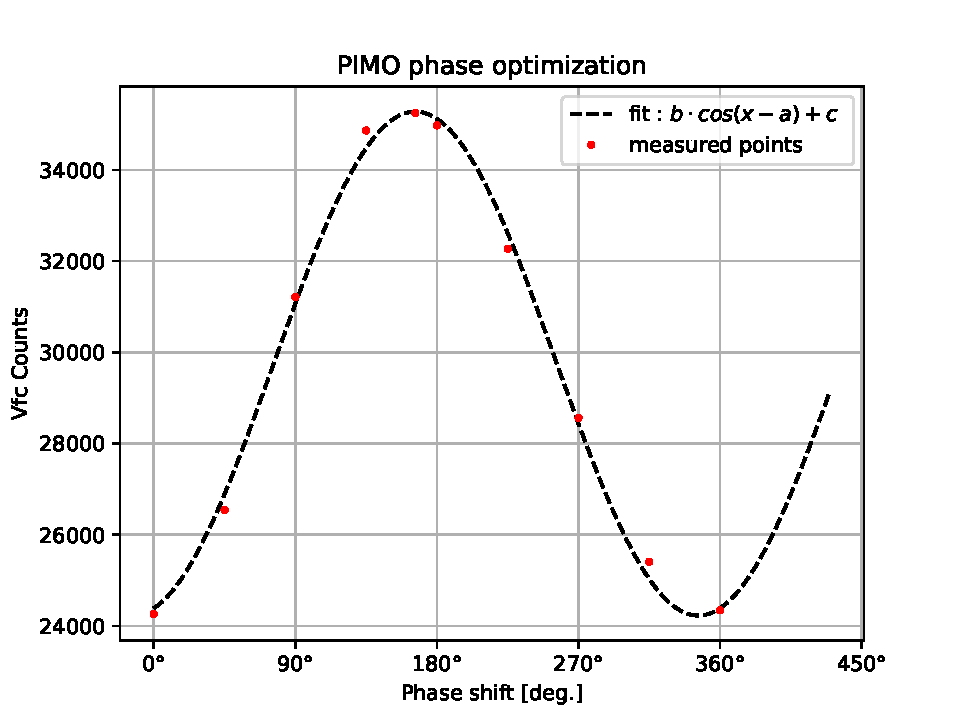
\includegraphics[width = 0.75\textwidth]{ExperimentalSetup/PIMOphase.pdf}
\caption{Plot of the output signal versus phase $\phi$. The phase optimization was done selecting the working point in correspondence of the peak.}
\label{fig:PIMO}
\end{figure}

The measurement of the $x,y$ position follows in principle the same procedure. In this case the $TM_{110}$ is acquired, because for this mode the $r_{shunt}$ is proportional to the beam position on the $x,y$ plane. The power absorbed by the antenna can be written:

\begin{equation}
P_{HF} = i^{2} r_{110} \frac{\kappa}{(1 + \kappa)^{2}} K x^{2}
\end{equation} 
 
The output signal, that is read by our setup, is proportional to the square root of the absorbed power:

\begin{equation}
U = \sqrt{P_{HF}} = constant \, \cdot \, i   \cdot x
\end{equation} 

The beam parameter are obtained by inverting the above formula 

\begin{equation} \label{eq:SignalToVfc}
x \propto \frac{\sqrt{P_{HF}}}{i}
\end{equation}

Where the exact conversion coefficients are not known, and are determined during the calibration phase, at the beginning of the beam time.
To measure the beam energy, a different approach is used. The energy monitor (ENMO) consists of 2 cavities in the RTM3. One is located in the last recirculation pipe, the other one on the part of the beam line, where the acceleration takes place. The two monitors are synchronized to the master oscillation and measure the phase of the bunches of electrons. During their travel from the first cavity to the second cavity, the beam passes through the magnet and does one half turn. If the energy is slightly higher, the radius of the turn will be slightly larger. This means that there is an extra time between the two bunches, that can be measured as a small phase shift in the $\SI{570}{\mega \electronvolt}$ recirculation. From this it is possible to obtain a value for the difference of the actual energy from the nominal energy.

\subsection{Beam stabilization}

The beam stabilization is an essential component of the experiment. The values of $A_{n}$ that we want to measure are in the order of  $10 \, ppm$, so it is important to reduce other contributions that can be related to variations in the beam parameters. The beam stabilization at MAMI is achieved with a control program. The beam monitors constantly measure the beam parameters and the control program receives the measurements from the monitors and calculates consequently the corrections to be performed. 
The beam position in the transverse plane is constantly adjusted by the magnets in the beam line. For the beam current and energy, the control program acts on the laser of the beam source and the klystrons in the three racetrack microtrons described in section \ref{ExperimentalHall}. Two types of stabilization are made by the control program: the first is made to avoid long term drifts by pulling back the beam back to nominal conditions every $\simeq \SI{10}{\second}$. Simultaneously, a fast stabilization prevents fast fluctuation, reacting quickly to every disturbance of the beam. 

\section{Electronics}
\subsection{Voltage to Frequency Converter} \label{VFCss} 

Some beam parameters are needed in order to take into account possible effects in the measurement of the transverse asymmetry. The relevant data are the position in the $(x,y)$ plane, the incident angles on the target, the current and energy of the beam. All this values are collected using the existing monitors. To collect the data from the monitors, single and multichannel, synchronous voltage-to-frequency converters (AD7742) are used. This devices contain an analog modulator that is able to convert the input voltage into an output pulse train, whose frequency is proportional to the input voltage. 

\begin{figure}[htb]
\centering
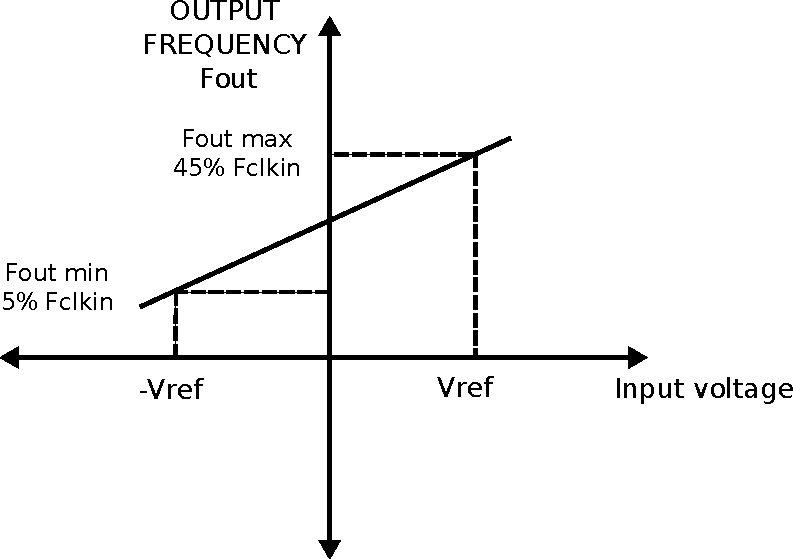
\includegraphics[width=0.5\textwidth]{ExperimentalSetup/Vfc.pdf}
\caption{Frequency versus Voltage}
\label{fig:VoltageToFrequency}
\vspace{10pt}
\end{figure}

The VFCs are powered with an external voltage of $\SI{5}{\volt}$. They measure an input voltage in the range of ($-V_{ref}$, $V_{ref}$). An external clock signal, with a frequency $F_{CLKIN} = \SI{5.88}{\mega \hertz}$ is created externally and synchronous to the gate-length.
The analog input signal is sampled with by a switched capacitor, with a rate that is equal to $F_{CLKIN}$.
The comparator produces a number pulses; the frequency of the output signal is proportional to the input voltage, with $-V_{ref}$ equal to $5 \% \cdot f_{CLKIN}$ and $+V_{ref}$ equal to $45 \% \cdot f_{CLKIN}$ \cite{VfcDatasheet}, where the first correspond to $\SI{0.0}{ \volt}$ in input and the second to $V_{ref}$ (see figure \ref{fig:VoltageToFrequency}). The data are acquired counting the number of pulses from the comparator, which are proportional to the frequency, so we can substitute to $f$ the number of pulses, and we end up with the equation \ref{eq:Vfc}

\begin{equation} \label{eq:Vfc}
V_{in} =  V_{ref}[2 \cdot \dfrac{N_{pulses} - 5 \% N_{CLKIN}}{40 \% N_{CLKN}} - 1]
\end{equation}

\subsection{Master Board}

The VFCs described in the previous section are measuring the beam parameters along the beam line. A figure of the beam line is in section \ref{XYpos}, where the various position of the monitors is shown.
The data collected by the VFCs are firstly acquired by the master board, in figure \ref{fig:MasterBoard}, and then sent to the A1 computer, which will produce the data package. The VFCs are synchronized by the master board clock, with a frequency of \SI{5.88}{\mega \hertz}. This is also the reference frequency for the VFCs output signal. 

\begin{figure}[hbtp]
\centering
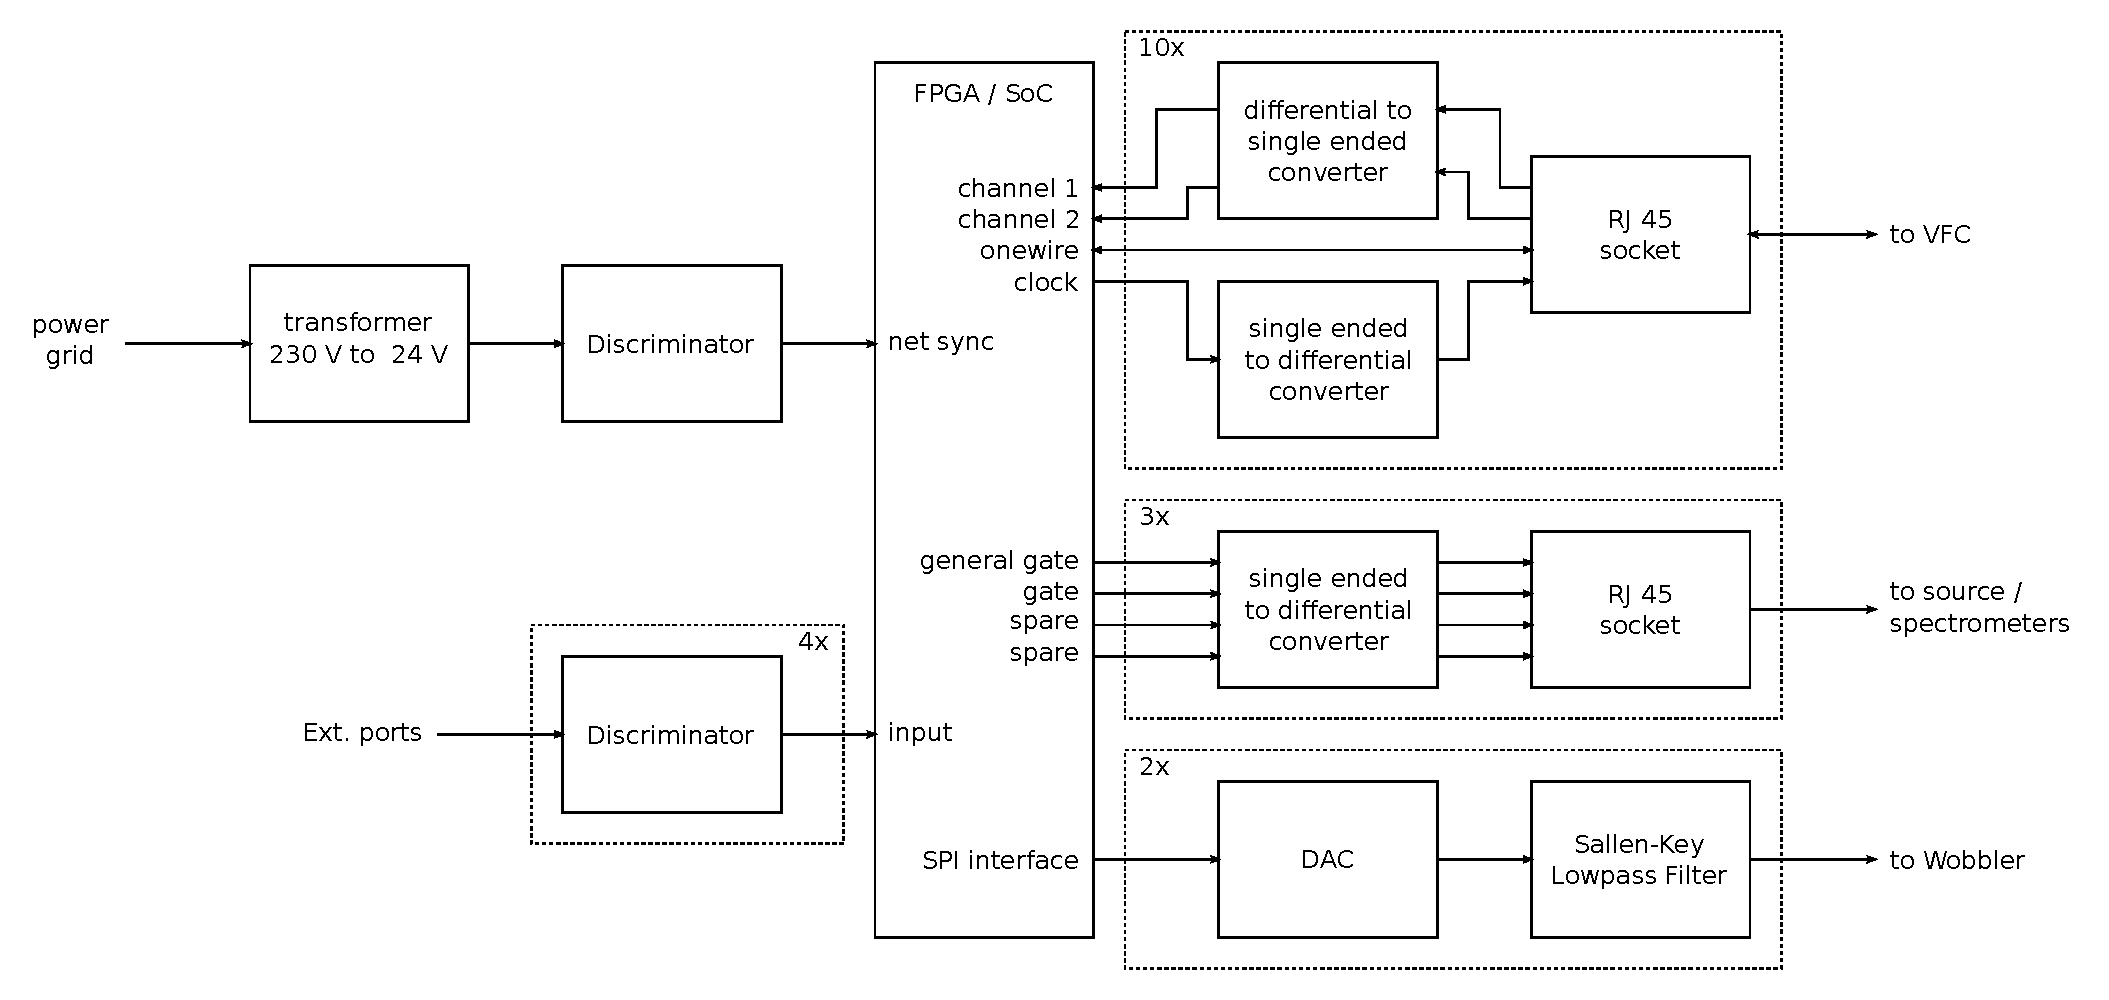
\includegraphics[width = \textwidth]{ExperimentalSetup/masterboard.pdf}
\caption{Scheme of the master-board, the device that coordinates all the electronics for the experiments, and send the data to the computer in the control room.}
\label{fig:MasterBoard}
\end{figure}

The \textit{onewire} is a special bus which will be used in future for temperature measurement in the VFC, to check if there are temperature drift and effects on the outputs signals. The master board sends also the gate length signal to the MAMI source, where the polarized beam is generated, and to the detectors, needed to communicate and synchronize the sub-events. 
For the experiment with the lead target, the master board will also control one of the magnets (\textit{wobbler 16}, in figure \ref{fig:BeamLine}). With the lead target, the beam position must be constantly changed so that the beam hitting point on the target is varies continuously, to avoid melting. The master board is synchronized to the power grid, is order to reduce possible systematics effect connected to the $\SI{50}{\hertz}$ frequency, as discussed in section \ref{FirstDescription}.

\subsection{Nino Board} \label{NINO}

The NINO board shown in \ref{fig:NinoBoard} is our data acquisition system for the PMT counts (see paper \cite{1352067}). It is made by $32$ analog input channels and it is powered with $\pm \SI{5}{\volt}$.
Each input channel receive a differential signal from the detector, and has attenuation circuit that reduces the amplitude of the input signal. After passing the attenuator, the signal is sent to the input stage of the NINO chip, a current-to-voltage converter, that produces an output signal whose amplitude is proportional to the total charge of the input signal.

\commento{
\begin{figure}[hbtp]
\centering
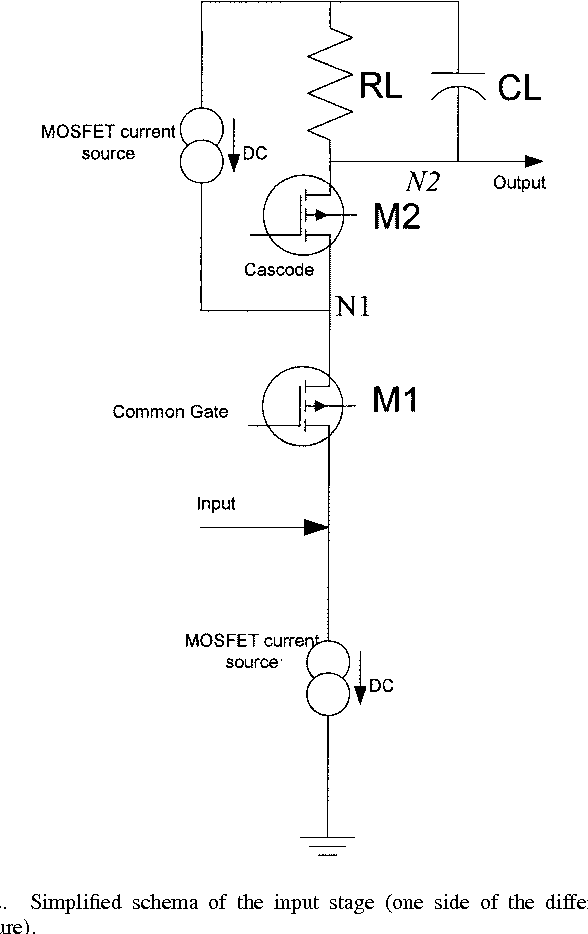
\includegraphics[width = 0.3\textwidth]{ExperimentalSetup/InputStage.png}
\caption{Input stage of the NINO chip. The input signal coming from the detector passes an attenuation circuit, and then are sent to the input stage, in this figure. The output, at node N2, is connected to the discriminator and an amplification stage.}
\label{fig:InputStage}
\end{figure}}

After passing the input stage, the signal goes through a block of 4 cascaded operational amplifiers that act as a discriminator with a programmable threshold. The NINO chip can handle signals coming from $8$ different channels and there are 4 NINO chips on each NINO board. 

\begin{figure}[!ht]
\centering
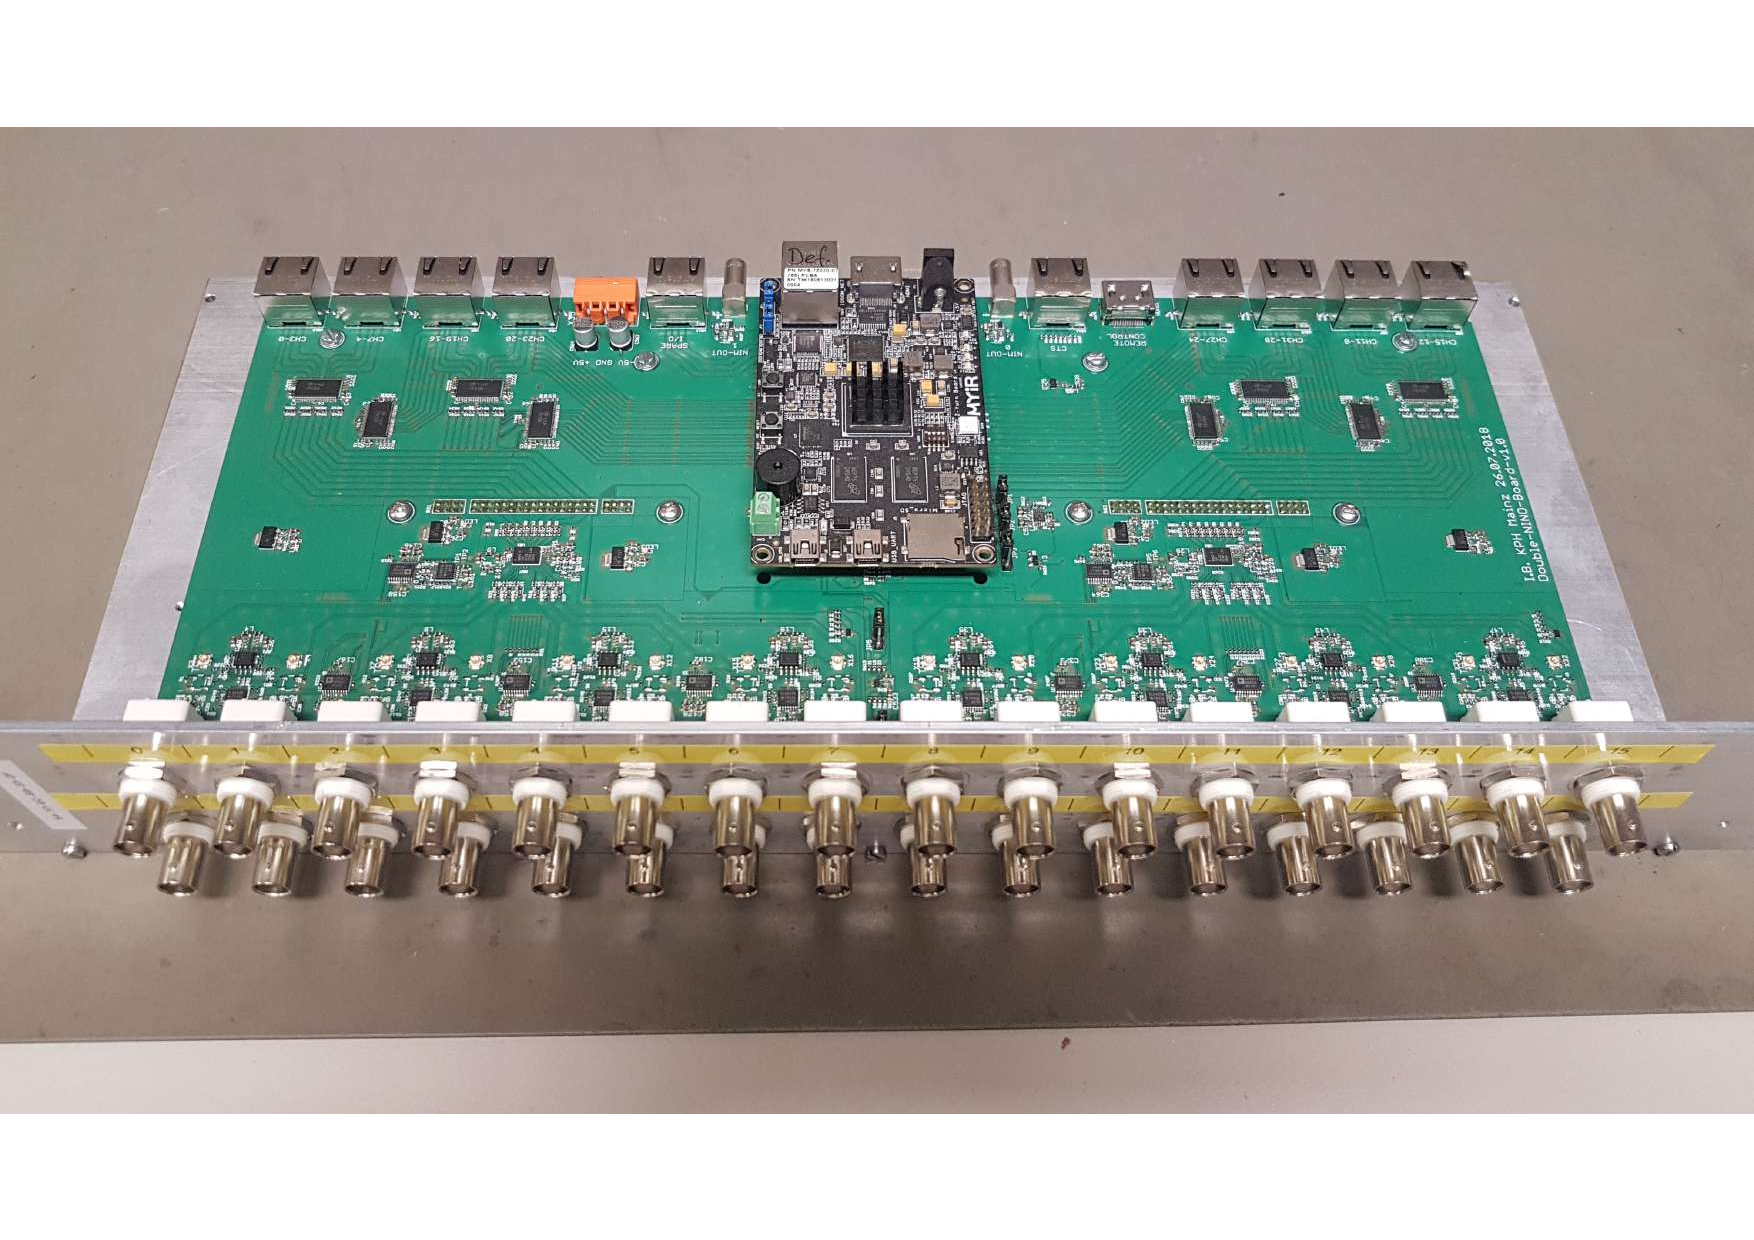
\includegraphics[width = 0.6\textwidth]{ExperimentalSetup/NINO.pdf}
\caption{Nino Board, The input channels are at the bottom of the figure.}
\label{fig:NinoBoard}
\end{figure}

The signal that arrives to the discriminator is proportional to the input charge of the signal coming from the detector, so in the end the NINO board is sensitive to the input charge. The discriminator threshold can be set in the range of (\SI{10}{\pico \coulomb}, \SI{100}{\pico \coulomb}). 
The output signal after the discriminator and the amplification block is a LVDS (low voltage differential signaling) with a fixed shape, and a width that is proportional to the input charge. Regarding the data acquisition system, two values are import to control the discriminator threshold and the attenuator, and are named \textit{Thr} and \textit{Att}, respectively. The NINO chip is designed in such a way that the \textit{Thr} value is shared by 4 adjacent channels. On the contrary each channel has is own value of \textit{Att}. Acting simultaneously on \textit{Thr} and \textit{Att} is possible to define a global threshold for each channel, individually.
These two parameters are set in the DAQ program, using 12 bit DACs, corresponding to interval of $(0 ; 4095)$. \textit{Thr} selects the threshold of the discriminator. The \textit{Att} value controls the input voltage of attenuator: the higher is the value of \textit{Att}, the lower is the attenuation of the signal.
Two Nino board are used in the experiment, one for detector A and one for detector B. For the experiment discussed in this thesis, we will use only 8 channel for detector A and 3 channel for detector B, since this is the number of the input signals coming from the two detectors. For the future experiments more channels will be used, splitting the analog input signal in 4, and sending it to 4 different input channel of the board. This is useful because changing individually the attenuation value, we can define 4 different thresholds for the same signal and compare different values of threshold, to study how the noise affects the measurement, finding the best compromise between signal to noise ratio. The \textit{Thr} and \textit{Att} selection is explained in chapter \ref{analysis}.



